% Traduzione italiana della versione in lavorazione dell'articolo (paper/main.tex su main).
% Il testo di riferimento resta quello inglese. Figure italiane correnti (report/fig), bibliografia corrente.
% Da aggiornare quando cambia paper/main.tex. Compilazione: make paper-it
\documentclass[preprint,12pt,authoryear]{elsarticle}

\usepackage[utf8]{inputenc}
\usepackage[T1]{fontenc}
\usepackage[italian]{babel}
\usepackage{lmodern}
\usepackage{amsmath,amssymb,amsthm}
\usepackage{booktabs}
\usepackage{graphicx}
\usepackage[colorlinks=true,linkcolor=blue!50!black,citecolor=blue!50!black,urlcolor=blue!50!black]{hyperref}

\graphicspath{{../../report/fig/}}
\newtheorem{proposition}{Proposizione}
\newcommand{\todo}[1]{\textcolor{red}{[#1]}}
\newcommand{\ndt}[1]{\footnote{[N.d.T.] #1}}

\journal{Structural Change and Economic Dynamics}

\begin{document}

\begin{frontmatter}

\title{Ciò che i senior non insegnano più: intelligenza artificiale e \emph{skill cliff}}

\author[aff1]{Federico Bassi}
\author[aff2]{Vincenzo Lio\corref{cor}}
\cortext[cor]{Autore di riferimento.}
\affiliation[aff1]{organization={\todo{Affiliazione}},country={\todo{Paese}}}
\affiliation[aff2]{organization={\todo{Affiliazione}},country={Italia}}

\begin{abstract}
\emph{Traduzione italiana della versione in lavorazione (\today); il testo di riferimento è quello inglese.}

\smallskip
Nel modello di crescita di \citet{Lucas1988} l'efficienza con cui i lavoratori accumulano capitale umano, $B$, è una costante. Nei lavori successivi dello stesso Lucas \citep{Lucas2009,LucasMoll2014}, la conoscenza si acquisisce negli incontri tra chi sa di più e chi sa di meno. Le prime evidenze secondo cui l'IA generativa riduce l'occupazione dei lavoratori all'inizio della carriera \citep{Brynjolfsson2025,HosseiniLichtinger2025} trasformano questa distinzione in una questione di politica economica: se l'IA sostituisce il lavoro dei junior, può anche eliminare le occasioni in cui i junior imparano dai senior \citep{Ide2026}. L'articolo sviluppa un modello ad agenti volutamente minimo, in cui $B$ non è assunto ma emerge dagli incontri tra junior e senior, e ne ricava due risultati principali. Primo, dimezzare in modo permanente le occasioni d'incontro lascia il capitale umano dei senior \emph{esattamente} invariato per dieci anni, cioè la distanza tra le soglie di esperienza di junior e senior, e poi lo erode del 6,7 per cento nel lungo periodo: una caduta ritardata che chiamiamo \emph{skill cliff}. Secondo, l'apprendimento dipende dal prodotto tra le occasioni d'incontro e la loro efficacia, così che un'IA che toglie compiti ai junior (meno incontri) o ai senior (incontri meno efficaci) riduce il capitale umano aggregato dello stesso 5,2 per cento dopo cinquant'anni, circa 0,11 punti percentuali di crescita l'anno, con effetti diversi sulla disuguaglianza. Ne seguono due conseguenze. Con una stima prudente della produttività dell'IA, la perdita di capitale umano assorbe circa l'86 per cento del guadagno di output; e un'impresa che non vede la perdita ritardata automatizza più del triplo della quota che sceglierebbe un pianificatore con un orizzonte di cinquant'anni, un eccesso invisibile su dieci anni. Un'identità aggregata esprime $B$ in funzione delle occasioni d'incontro, della capacità di mentoring e della distribuzione della conoscenza, e può essere usata nei modelli di crescita a una equazione.
\end{abstract}

\begin{keyword}
Capitale umano \sep Diffusione della conoscenza \sep Intelligenza artificiale \sep Modello ad agenti \sep Mentoring \sep Skill cliff
\JEL C63 \sep J24 \sep O33 \sep O41 \sep J11
\end{keyword}

\end{frontmatter}

% ---------------------------------------------------------------------------
\section{Introduzione}

L'IA generativa sta riducendo l'occupazione dei giovani nelle occupazioni più esposte, lasciando sostanzialmente invariata quella dei senior \citep{Brynjolfsson2025,HosseiniLichtinger2025}. L'effetto di primo round riguarda il mercato del lavoro. Quello di secondo round riguarda il capitale umano: i junior imparano gran parte del mestiere lavorando accanto ai senior, e i junior che non vengono assunti oggi sono i senior che non ci saranno a insegnare fra quindici anni. L'articolo si chiede che cosa succede al capitale umano di un'economia quando diventano più rare le occasioni in cui chi sa incontra chi impara, e quanto tempo passa prima che qualcuno se ne accorga.

Sviluppiamo un modello ad agenti (ABM) in cui $B$ è una proprietà emergente degli incontri tra junior e senior, nello spirito dell'uso dei metodi ad agenti per microfondare dinamiche aggregate in \citet{Bassi2022} e \citet{RailsbackGrimm2011}. Il modello è volutamente minimo: i lavoratori seguono regole fisse e non fanno scelte economiche. È una scelta di metodo: isoliamo il canale del capitale umano, ne caratterizziamo le proprietà, anche analiticamente, e rinviamo a lavori futuri le risposte di comportamento di imprese e lavoratori. Il modello riproduce un profilo salariale per età concavo e una quota di apprendimento dai colleghi coerente con \citet{Jarosch2021}, e dà due risultati principali. Primo, una riduzione permanente delle occasioni d'incontro produce una \emph{skill cliff}: il capitale umano dei senior resta esattamente invariato per $s_S - s_J$ anni, dove $s_J$ e $s_S$ sono le soglie di esperienza di junior e senior, e poi cala man mano che le coorti formate con meno incontri diventano gli insegnanti delle successive. Secondo, l'apprendimento dagli incontri dipende dal prodotto tra occasioni ed efficacia, così che che cosa significa sostituire conta quanto chi viene sostituito: togliere compiti ai junior (meno incontri) o ai senior (incontri meno efficaci) costa lo stesso capitale umano ma differisce per disuguaglianza e per guadagno di output nella transizione, mentre i junior che perdono il posto rinviano la propria formazione invece di perderla. Ne seguono due conseguenze per l'IA: la corsa tra la produttività dell'IA e l'erosione del capitale umano può essere persa anche quando l'IA aumenta l'output nel breve periodo, e le imprese che non internalizzano la trasmissione della conoscenza automatizzano più di quanto sia socialmente ottimale, di una quantità che diventa visibile solo dopo il ritardo di trasmissione. Lungo la strada ricaviamo un'identità aggregata per $B$ che può essere usata per rendere endogena l'efficienza dell'apprendimento nei modelli di crescita a una equazione come quello di \citet{Lucas1988}.

La domanda si collega all'efficienza dell'apprendimento, $B$, nel modello di crescita di \citet{Lucas1988}, dove il capitale umano cresce come
\begin{equation}\label{eq:lucas}
\dot h = B\,(1-u)\,h,
\end{equation}
con $1-u$ la quota di tempo dedicata all'apprendimento. Nel 1988 $B$ è una costante. Eppure due persone che dedicano lo stesso tempo all'apprendimento imparano a velocità molto diverse se il contesto è diverso: un programmatore junior il cui codice viene rivisto da un ingegnere senior ha un $B$ più alto di uno il cui unico interlocutore è un motore di ricerca. Lo stesso Lucas ha poi modellato la conoscenza come acquisita negli incontri tra chi sa di più e chi sa di meno \citep{Lucas2009,LucasMoll2014}, e gli studi empirici trovano che l'apprendimento dai colleghi vale il 4--9 per cento della retribuzione \citep{Jarosch2021,Herkenhoff2024}. Se $B$ è un parametro, una tecnologia che cambia l'organizzazione del lavoro lascia intatta l'efficienza dell'apprendimento; se $B$ emerge dagli incontri, una tecnologia che riduce gli incontri riduce $B$ stesso. \citet{Ide2026} mostra, in un modello a generazioni sovrapposte, che automatizzare i compiti d'ingresso taglia il canale attraverso cui la conoscenza tacita passa alla generazione successiva, che il mercato automatizza più di quanto sia socialmente ottimale, e che la crescita di lungo periodo del reddito pro capite può ridursi di 0,05--0,35 punti percentuali l'anno.

La letteratura presenta però tre lacune. L'efficienza dell'apprendimento è di solito trattata come un parametro, anche dove le sue microfondazioni sono esplicitamente sociali. Gli effetti dell'IA sul mercato del lavoro sono misurati all'impatto, mentre il canale di trasmissione opera con un ritardo di una generazione professionale: nessuno può ancora osservare il capitale umano dei senior del 2040. E i tempi di questo ritardo, e le condizioni in cui meno incontri si traducono in una caduta del capitale umano aggregato, non sono stati, per quanto ci risulta, caratterizzati.

Il resto dell'articolo è organizzato come segue. La sezione~\ref{sec:background} ripercorre il quadro teorico. La sezione~\ref{sec:model} presenta il modello così come è implementato. La sezione~\ref{sec:results} riporta le simulazioni di base e un esperimento di meccanismo che isola il canale degli incontri. La sezione~\ref{sec:aggregate} ricava le implicazioni per la modellistica aggregata. La sezione~\ref{sec:ai} introduce l'IA. La sezione~\ref{sec:conclusions} discute le politiche e conclude.

% ---------------------------------------------------------------------------
\section{Quadro teorico e motivazione}\label{sec:background}

\subsection{L'efficienza dell'apprendimento: da parametro a processo}

In \citet{Lucas1988} il parametro $B$ determina il tasso di crescita bilanciata dell'economia e, lungo il sentiero di sella, la velocità con cui l'economia vi si avvicina. La teoria del capitale umano \citep{Becker1964,Mincer1974} e i modelli del ciclo di vita di investimento in capitale umano \citep{BenPorath1967,Rosen1972} spiegano perché l'apprendimento individuale cala con l'età, e quindi perché i profili empirici dei redditi per età sono concavi \citep{MurphyWelch1990,Lagakos2018}; ma anche loro trattano la produttività dell'apprendimento come data. In \citet{LucasMoll2014} il parametro è sostituito da un processo: la distribuzione della conoscenza nella popolazione è la variabile di stato, e la crescita dipende da quanto spesso le persone si incontrano, da chi incontrano, e da se la differenza di conoscenza tra loro è abbastanza grande da rendere fruttuoso l'incontro. $B$ diventa il risultato endogeno della struttura degli incontri tra lavoratori: alto quando i junior incontrano spesso senior più capaci, basso quando quegli incontri scompaiono. La stessa logica è alla base dei modelli di diffusione delle idee attraverso incontri casuali \citep{AlvarezBueraLucas2013,PerlaTonetti2014,BueraOberfield2020} e del trasferimento di capitale umano dai lavoratori esperti a quelli inesperti \citep{JovanovicNyarko1995}. Dentro le organizzazioni, le gerarchie della conoscenza permettono a chi sa meno di attingere a chi sa di più \citep{Garicano2000,GaricanoRossiHansberg2006}, e le interazioni con colleghi più produttivi aumentano la produttività individuale \citep{Akcigit2018}. Un filone diverso, sul capitale umano d'annata, mostra che le competenze legate a una tecnologia perdono valore quando la tecnologia cambia \citep{ChariHopenhayn1991,Violante2002}; nel modello tocchiamo questo canale solo attraverso la familiarità con l'IA (sezione~\ref{sec:ai}).\footnote{La corrispondenza tra l'evidenza e la nostra misura è approssimata: \citet{Jarosch2021} misurano l'apprendimento da tutti i colleghi in quota della retribuzione di tutti i lavoratori, mentre noi misuriamo l'apprendimento dei junior dai senior in quota del salario dei junior.}

\subsection{Automazione, lavoro d'ingresso e il canale dell'apprendistato}

La conoscenza tacita è diversa da quella codificata: non sta nei manuali e non si trasmette con una presentazione, ma si acquisisce con la pratica situata, l'errore e la correzione in tempo reale. \citet{Ide2026} individua due forze attraverso cui l'IA ne erode la trasmissione. Dal lato dell'offerta, automatizzare i compiti d'ingresso riduce le occasioni di apprendistato che gli esperti offrono. Dal lato della domanda, i co-pilot basati sull'IA compensano in parte i mentori mancanti, ma riducono anche lo sforzo che i principianti mettono nell'imparare facendo: consegnano il risultato senza costruire la capacità, e la capacità è proprio ciò che serve per diventare il senior che insegnerà alla generazione successiva.

Le evidenze disponibili misurano solo l'effetto di primo round. L'occupazione dei 22--25enni nelle occupazioni esposte all'IA è calata del 13--16 per cento rispetto a quella dei lavoratori più anziani \citep{Brynjolfsson2025}, e le imprese che adottano l'IA generativa assumono meno junior \citep{HosseiniLichtinger2025}. Nella visione del progresso tecnico per compiti \citep{AutorLevyMurnane2003,AcemogluAutor2011}, sono le occupazioni con la quota più alta di compiti esposti ai modelli linguistici \citep{Eloundou2024}. Le evidenze sperimentali aggiungono un elemento: l'IA generativa aumenta la produttività soprattutto dei lavoratori meno esperti \citep{NoyZhang2023,DellAcqua2023,BrynjolfssonLiRaymond2025}, e può quindi fare anche da tutor; la sezione~\ref{sec:conclusions} torna su questo canale. L'effetto di secondo round, sul capitale umano dei senior futuri, per costruzione non è ancora osservabile. Serve un modello per disciplinare le aspettative al riguardo.

\subsection{Sostituzione, complementarità e direzione}

\citet{Acemoglu2024} stima guadagni di produttività aggregati modesti dall'IA nel prossimo decennio e sostiene che la sua direzione conta: l'IA può essere usata per potenziare i lavoratori o per sostituirli, e l'industria sta scegliendo la seconda opzione perché riduce il costo del lavoro nel breve periodo \citep[si veda anche][]{AcemogluRestrepo2019}. Nel quadro dell'Eq.~\eqref{eq:lucas} la distinzione ha conseguenze precise: un'IA complementare può aumentare $B$ rendendo l'apprendimento più efficiente, mentre un'IA sostitutiva lo riduce svuotando i contesti in cui l'apprendimento avviene. Acemoglu ha ragione sul fatto che la direzione conta, ma l'analisi si ferma al breve periodo e ai compiti direttamente automatizzabili: non coglie il meccanismo intergenerazionale. Il problema non è solo quanti posti di lavoro scompaiono oggi, ma quanta conoscenza tacita non viene trasmessa domani.

Il collegamento tra questi tre filoni (Lucas e Moll sulla natura sociale di $B$, Ide sull'automazione come distruttrice di incontri, Acemoglu sulla direzione del progresso tecnico) è una nostra interpretazione, non un risultato di nessuno di essi. Il modello della prossima sezione è costruito per verificare se regge quantitativamente.

\subsection{Modelli ad agenti con competenze}

La macroeconomia ad agenti include da tempo lavoratori eterogenei e progresso tecnico \citep{Tesfatsion2006,DawidDelliGatti2018}. Nel modello Eurace@Unibi le competenze dei lavoratori determinano la diffusione della tecnologia tra regioni \citep{Dawid2012}; nella famiglia K+S il progresso tecnico interagisce con le istituzioni del mercato del lavoro e con la domanda aggregata \citep{Dosi2010,Dosi2017}. Questi modelli inseriscono i lavoratori in un'economia completa, con imprese, prezzi e credito. Noi prendiamo la strada opposta: un modello minimo del solo canale del capitale umano, in cui gli agenti seguono regole fisse e non fanno scelte economiche. È una scelta di metodo, non un'omissione. Isolare il meccanismo di trasmissione permette di caratterizzarne le proprietà analiticamente (sezione~\ref{sec:aggregate}) e di trasferirle, come mattone, a modelli più ricchi; le risposte di comportamento di imprese e lavoratori sono rinviate a lavori futuri.

% ---------------------------------------------------------------------------
\section{Il modello}\label{sec:model}

\subsection{Agenti e demografia}

L'economia è popolata da $N=5.000$ lavoratori indicizzati da $i$; ogni periodo corrisponde a un anno. Il lavoratore $i$ è caratterizzato dall'età $a_{i,t}$, dagli anni di esperienza $s_{i,t}$, da un livello di qualifica $q_i\in\{L,H\}$ e dal capitale umano $h_{i,t}$. All'inizio di ogni periodo tutti i lavoratori invecchiano di un anno, $a_{i,t}=a_{i,t-1}+1$, e chi era occupato l'anno precedente guadagna un anno di esperienza, $s_{i,t}=s_{i,t-1}+1$ (senza IA tutti sono occupati; la non occupazione compare solo nella sezione~\ref{sec:ai}); chi raggiunge l'età di pensionamento $\bar a=65$ esce ed è sostituito uno a uno da un entrante, così che $N$ resta costante.\footnote{Una variante con la piramide per età italiana, in cui $N$ varia nel tempo, è rinviata a uno studio dedicato.} Un entrante è qualificato con probabilità $q=0{,}3$, entra con $s=0$ a 25 anni se qualificato e a 20 altrimenti, ed estrae
\begin{equation}\label{eq:entry}
h_{i,0} = \bar h_0(q_i)\, e^{\varepsilon_i}, \qquad \varepsilon_i \sim \mathcal N\!\left(-\tfrac{\sigma^2}{2},\sigma^2\right),
\end{equation}
con $\bar h_0(L)=1$, $\bar h_0(H)=1{,}5$ e $\sigma=0{,}2$. I ruoli sono definiti dall'esperienza e non dall'età: il lavoratore $i$ è \emph{junior} se $s_{i,t} < s_J$ e \emph{senior} se $s_{i,t} \ge s_S$, con $s_J=5$ e $s_S=15$.

\subsection{Incontri}

I junior imparano dai senior del proprio gruppo di qualifica $g\in\{L,H\}$: si impara da chi fa lo stesso lavoro. Siano $J_{g,t}$ e $S_{g,t}$ il numero di junior e di senior nel gruppo $g$. Ogni senior può seguire al massimo $\kappa$ junior l'anno, così che il numero di incontri è $\min(pJ_{g,t},\kappa S_{g,t})$ e la probabilità che un junior incontri un senior è
\begin{equation}\label{eq:peff}
p^{\mathrm{eff}}_{g,t} = \min\!\left(p,\ \kappa \frac{S_{g,t}}{J_{g,t}}\right).
\end{equation}
Un junior $j$ che incontra un senior $k$, estratto in modo uniforme tra i senior dello stesso gruppo, guadagna
\begin{equation}\label{eq:meeting}
\Delta h^{\mathrm{inc}}_{j,t} = \beta \max\left(0,\ h_{k,t}-h_{j,t}\right),
\end{equation}
come in \citet{LucasMoll2014}: il guadagno è proporzionale al divario di conoscenza, e da un senior che sa meno non si disimpara nulla. Il senior non sostiene costi.

\subsection{Apprendimento autonomo e obsolescenza}

Tutti i lavoratori imparano anche in modo autonomo, a un tasso che cala con l'esperienza come in \citet{BenPorath1967}, e perdono per obsolescenza una frazione $d$ della propria conoscenza:
\begin{equation}\label{eq:aut}
\Delta h^{\mathrm{aut}}_{i,t} = \left[\delta(s_{i,t})-d\right] h_{i,t}, \qquad \delta(s) = \delta_0 \max\!\left(0,\ 1-\frac{s}{S_h}\right).
\end{equation}
Entrambe le componenti sono calcolate sul capitale umano di inizio periodo e applicate insieme, $h_{i,t+1}=h_{i,t}+\Delta h^{\mathrm{inc}}_{i,t}+\Delta h^{\mathrm{aut}}_{i,t}$; $h$ resta non negativo perché $d<1$.

\subsection{Output, salari ed efficienza emergente dell'apprendimento}

L'output è $Y_t=\sum_i h_{i,t}$ e i salari sono pari ai prodotti marginali, $w_i = h_i$.\footnote{Con l'IA l'output diventa $Y_t = f(\sum_i h_{i,t}, A_t)$.} L'efficienza emergente dell'apprendimento è misurata come tasso medio di crescita del capitale umano dei junior,
\begin{equation}\label{eq:B}
B_t = \underbrace{\frac{1}{J_t}\sum_{j}\frac{\Delta h^{\mathrm{inc}}_{j,t}}{h_{j,t}}}_{B^{\mathrm{inc}}_t} + \underbrace{\frac{1}{J_t}\sum_{j}\frac{\Delta h^{\mathrm{aut}}_{j,t}}{h_{j,t}}}_{B^{\mathrm{aut}}_t},
\end{equation}
che corrisponde a $\dot h/h = B(1-u)$ nell'Eq.~\eqref{eq:lucas} con il tempo dedicato all'apprendimento normalizzato a uno.

\subsection{Calibrazione e implementazione}

La tabella~\ref{tab:params} riporta i valori dei parametri. I parametri demografici riflettono il mercato del lavoro italiano; $\beta$ è scelto in modo che $B^{\mathrm{inc}}$ cada nell'intervallo stimato da \citet{Jarosch2021}; $(\delta_0,S_h,d)$ sono scelti per produrre un profilo salariale per età che cresce lentamente, raggiunge il picco tardi e cala solo di poco, come nel settore privato italiano. Il modello è implementato in Python vettorizzato; ogni simulazione include un burn-in di 300 anni, e le statistiche sono medie su 30 repliche con seed indipendenti e intervalli di confidenza al 95\% \citep[sul numero di repliche si veda][]{Lee2015}. La calibrazione è indiretta: i parametri sono scelti per riprodurre alcuni fatti stilizzati, e le altre proprietà del modello non sono obiettivi \citep{Windrum2007,Fagiolo2007}. Poiché diversi parametri sono scelti a mano, l'appendice~\ref{app:sobol} riporta un'analisi di sensibilità globale dei risultati principali. Gli scenari condividono i numeri casuali replica per replica. Una reimplementazione indipendente delle stesse regole in Mesa \citep{Kazil2020}, con un oggetto per agente, dà risultati statisticamente equivalenti entro $\pm1$ per cento (appendice~\ref{app:docking}), una forma di \emph{docking} tra modelli \citep{Axtell1996}; una terza implementazione in NetLogo \citep{Wilensky1999}, che copre tutti gli scenari con IA, coincide entro lo 0,25 per cento. Una descrizione completa secondo il protocollo ODD è nell'appendice~\ref{app:odd}. Codice e dati sono disponibili su \url{https://github.com/ViciusLio/skill-cliff-abm}.

\begin{table}[t]\centering\small
\caption{Parametri del modello di base.}\label{tab:params}
\begin{tabular}{@{}l l p{0.29\linewidth} p{0.24\linewidth}@{}}
\toprule
Parametro & Valore & Descrizione & Fonte / criterio \\
\midrule
$N$ & 5.000 & lavoratori & --- \\
età d'ingresso & 20 / 25 & non qualificati / qualificati & i laureati italiani entrano tardi \\
$\bar a$ & 65 & età di pensionamento & età effettiva di uscita, Italia 2024 \\
$q$ & 0,30 & quota di entranti qualificati & quota di laureati, 25--34 anni \\
$\bar h_0(L),\bar h_0(H)$ & 1,0 / 1,5 & capitale umano medio d'ingresso & normalizzazione \\
$\sigma$ & 0,20 & dispersione di $h$ all'ingresso & arbitrario \\
$s_J$ / $s_S$ & 5 / 15 & soglie junior / senior & evidenza sui lavori d'ingresso \\
$p$ & 0,60 & probabilità d'incontro & arbitrario (con $\beta$) \\
$\kappa$ & 0,20 & capacità di mentoring & arbitrario \\
$\beta$ & 0,10 & efficacia dell'incontro & $B^{\mathrm{inc}}\in[4\%,9\%]$ \\
$\delta_0, S_h, d$ & 0,04 / 50 / 0,012 & apprendimento autonomo, obsolescenza & profilo concavo \\
\bottomrule
\end{tabular}
\end{table}

% ---------------------------------------------------------------------------
\section{Risultati delle simulazioni}\label{sec:results}

\subsection{Il caso base: fatti stilizzati}

Il caso base riproduce un profilo salariale per età concavo (figura~\ref{fig:profile}). I salari raggiungono il picco dopo 34--35 anni di esperienza in entrambi i gruppi di qualifica, a un livello pari a 1,84 volte il salario d'ingresso, e calano del 3,6 (non qualificati) e dello 0,8 (qualificati) per cento prima del pensionamento. L'efficienza emergente dell'apprendimento è $B=0{,}0693$ (IC al 95\% $[0{,}0692;\ 0{,}0694]$), di cui $B^{\mathrm{inc}}=0{,}0429$, cioè il 62 per cento, viene dagli incontri (figura~\ref{fig:B}, pannello a). Il rapporto tra senior e junior è 5,71, così che la capacità di mentoring non è vincolante nello stato stazionario ($p^{\mathrm{eff}}=p$).

Vanno segnalate due discrepanze. Primo, i profili dei due gruppi di qualifica hanno la stessa pendenza, mentre l'evidenza indica che sono più ripidi per i più istruiti \citep{Lagakos2018}; riprodurlo richiederebbe un tasso di apprendimento autonomo diverso per qualifica, che lasciamo fuori per mantenere il modello essenziale. Secondo, il Gini dei salari (0,155) è molto più basso dei valori osservati, perché nel modello il capitale umano è l'unico determinante dei salari. Nessuno dei due è un obiettivo della calibrazione.

\begin{figure}[t]\centering
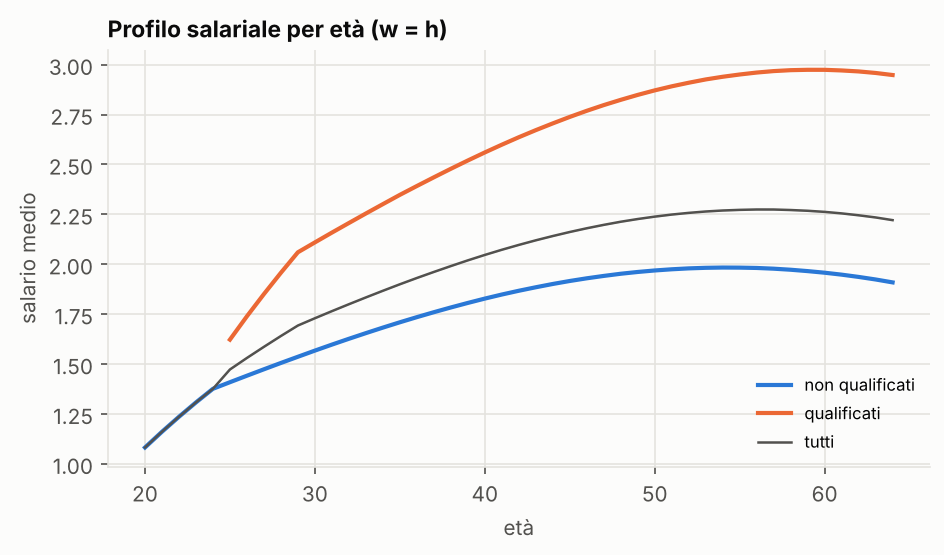
\includegraphics[width=.62\linewidth]{fig3_profilo_salariale.png}
\caption{Profilo salariale per età nel caso base. Media su 30 repliche e 60 anni; le bande sono intervalli di confidenza al 95\%.}\label{fig:profile}
\end{figure}

\subsection{La skill cliff: un esperimento di meccanismo}

Per isolare il canale attraverso cui opererà l'IA, dimezziamo $p$ in modo permanente dall'anno 10, tenendo fermo tutto il resto.\footnote{Non è uno scenario di IA: è la dinamica comparata del solo canale degli incontri.} La figura~\ref{fig:cohorts} riporta il capitale umano medio per classe d'età. La risposta è immediata per i junior, il cui capitale umano è più basso del 5,7 per cento dopo quattro anni. Per i senior la risposta è ritardata: il loro capitale umano medio resta \emph{esattamente} invariato per dieci anni, comincia a scendere all'undicesimo, è più basso del 3,6 per cento dopo 25 anni e del 6,7 per cento nel nuovo stato stazionario, mentre l'output cala del 7,2 per cento. La perdita si propaga lungo la distribuzione per età come un'onda: supera lo 0,5 per cento subito per i lavoratori di 20--29 anni, e dopo circa 4, 14, 24 e 33 anni per le classi d'età successive.

Il sentiero dell'efficienza dell'apprendimento non è monotono (figura~\ref{fig:B}, pannello b). $B^{\mathrm{inc}}$ si dimezza all'impatto, da 0,043 a 0,021; poi risale a 0,025 nei due decenni successivi, perché i junior partono da livelli più bassi e il divario dai loro senior si allarga; e cala di nuovo, a 0,020 dopo 50 anni, quando i senior formati con meno incontri diventano gli insegnanti. L'efficienza dell'apprendimento eredita la storia degli incontri: non è un parametro ma una variabile di stato. Infine, il Gini dei salari sale da 0,155 a 0,165 (figura~\ref{fig:gini}): gli incontri comprimono la disuguaglianza avvicinando i junior ai senior.

\begin{figure}[t]\centering
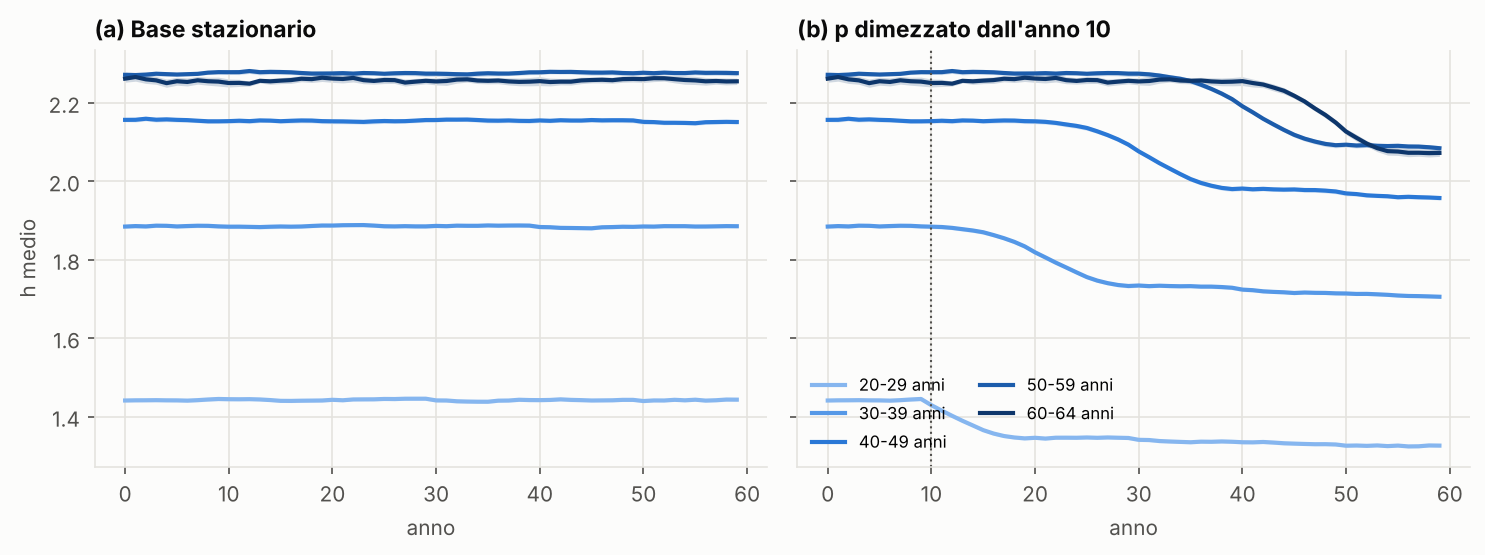
\includegraphics[width=\linewidth]{fig1_h_per_classe_eta.png}
\caption{Capitale umano medio per classe d'età. (a) Caso base. (b) Probabilità d'incontro dimezzata dall'anno 10. Media su 30 repliche; le bande sono intervalli di confidenza al 95\%.}\label{fig:cohorts}
\end{figure}

\begin{figure}[t]\centering
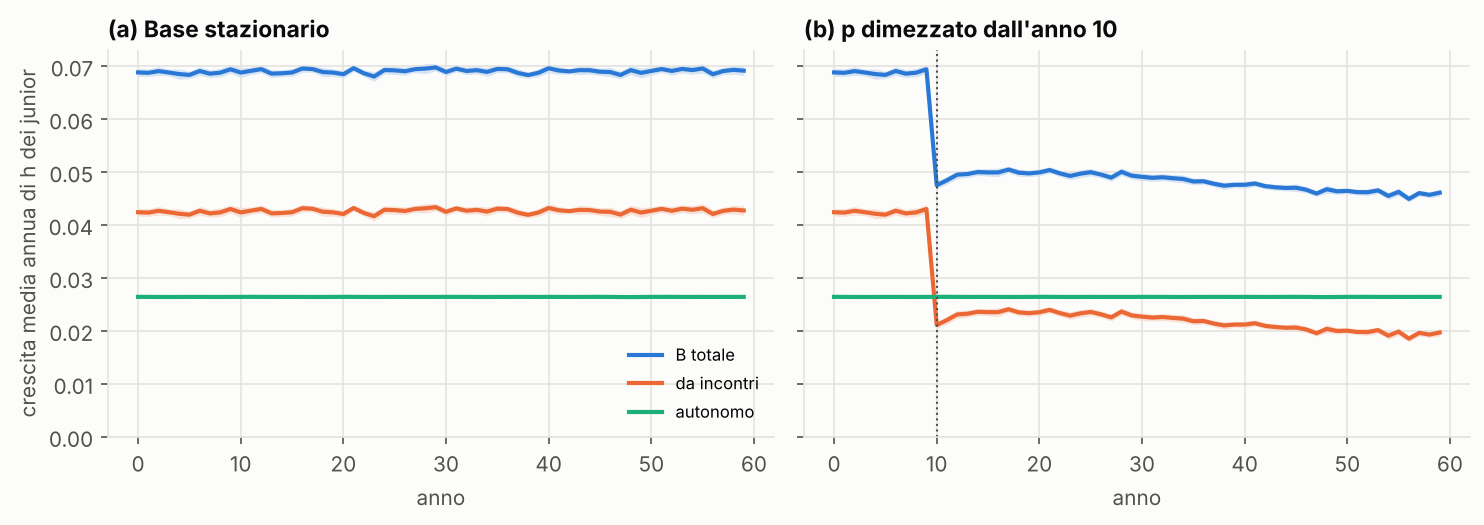
\includegraphics[width=\linewidth]{fig2_B_emergente.png}
\caption{Efficienza emergente dell'apprendimento dei junior e sua scomposizione.}\label{fig:B}
\end{figure}

\begin{figure}[t]\centering
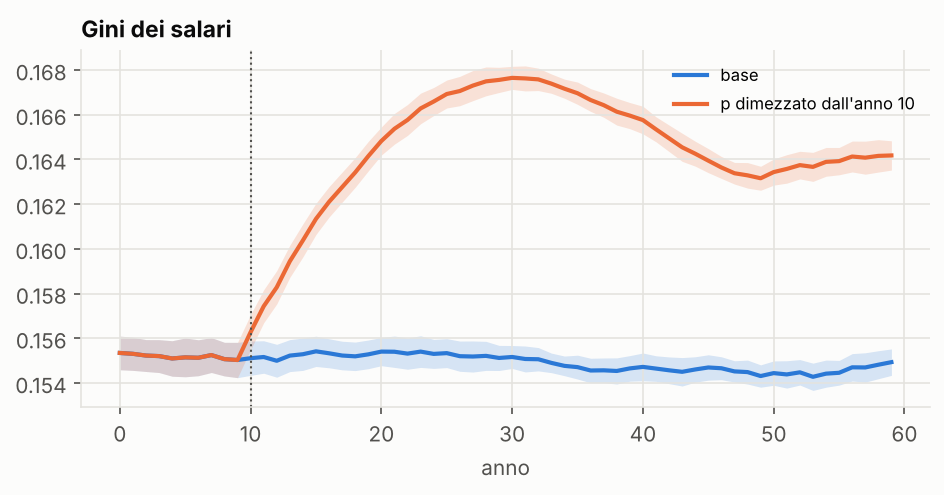
\includegraphics[width=.62\linewidth]{fig4_gini.png}
\caption{Coefficiente di Gini dei salari.}\label{fig:gini}
\end{figure}

\subsection{Capacità di mentoring e robustezza}

La figura~\ref{fig:sens} mostra $B^{\mathrm{inc}}$ e il capitale umano medio dei senior in funzione di $p$ per diversi valori di $\kappa$. Entrambi crescono più che linearmente in $p$, per il meccanismo cumulativo descritto sopra, finché il vincolo di capacità dell'Eq.~\eqref{eq:peff} non diventa attivo; oltre quel punto la domanda aggiuntiva di incontri è razionata. Nel caso base il vincolo diventa attivo solo se $S/J$ scende sotto $p/\kappa=3$, cioè dopo una forte riduzione del numero di senior rispetto ai junior.

Con soglie $s_J=10$ e $s_S=20$, $B$ scende a 0,057 perché il gruppo dei junior include lavoratori più lontani dall'ingresso, ma gli effetti di lungo periodo del dimezzamento di $p$ sono simili ($-6{,}6$ per cento per il capitale umano dei senior, $-7{,}2$ per cento per l'output) e il ritardo di trasmissione è ancora di 11 anni: dipende dalla distanza tra le soglie, non dal loro livello.

\begin{figure}[t]\centering
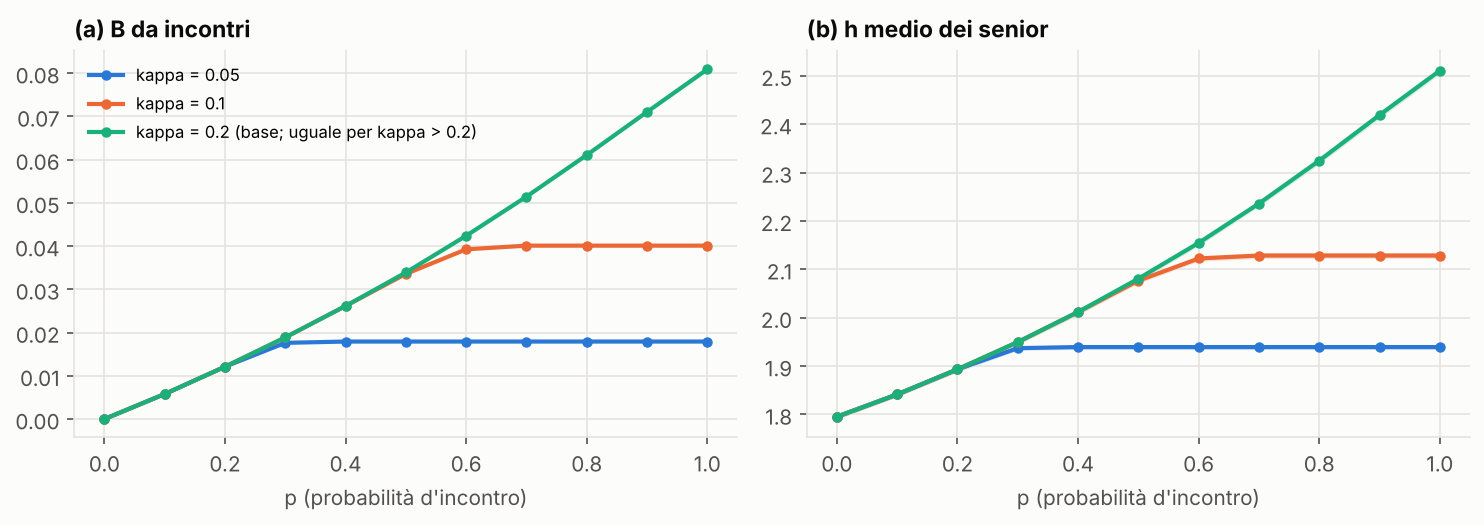
\includegraphics[width=\linewidth]{fig5_sensibilita_p_kappa.png}
\caption{Sensibilità alla probabilità d'incontro $p$ e alla capacità di mentoring $\kappa$ (10 repliche per punto).}\label{fig:sens}
\end{figure}

\subsection{Una regolarità non usata nella calibrazione: le coorti che entrano in una recessione}

La calibrazione ha come obiettivi il profilo salariale per età e la quota di apprendimento dai colleghi. Una regolarità che non è un obiettivo è la persistenza delle perdite salariali delle coorti che entrano nel mercato del lavoro durante una recessione. Simuliamo una recessione di due anni in cui una quota $u$ di chi cerca il primo lavoro resta non occupata; come nella sezione~\ref{sec:ai}, un anno senza lavoro non conta come esperienza, così che si ritenta l'anno dopo. Nessun'altra regola cambia. Poiché gli scenari condividono i numeri casuali, confrontiamo gli stessi lavoratori con e senza recessione, e misuriamo il salario medio delle coorti entrate durante la recessione rispetto al loro controfattuale (figura~\ref{fig:recession}).

La perdita iniziale è proporzionale alla quota di entranti rimasti fuori: circa lo 0,9 per cento del salario medio della coorte per ogni 10 per cento della coorte che resta senza lavoro per un anno. La sua persistenza non dipende dall'intensità dello shock. Dopo cinque anni, quando i membri della coorte non colpiti smettono di essere junior mentre chi è entrato tardi impara ancora dai senior, la perdita scende a circa il 40 per cento del suo massimo. Poi cala lentamente, perché chi ha meno esperienza impara in autonomia un po' più in fretta: resta il 34--35 per cento della perdita massima dopo dieci anni, il 30 per cento dopo quindici e il 15 per cento dopo trenta. Le evidenze empiriche racchiudono questo andamento. Nei dati amministrativi canadesi le perdite svaniscono dopo otto-dieci anni \citep{Oreopoulos2012}; per i laureati americani la perdita è ancora di circa il 2,5 per cento quindici anni dopo una perdita iniziale del 6--7 per cento per punto di disoccupazione \citep{Kahn2010}, cioè circa il 40 per cento del valore iniziale. Il modello è vicino alla seconda stima. Il livello della perdita, invece, non è confrontabile: nel modello l'unico canale è l'esperienza persa da chi resta senza lavoro, mentre le stime includono la qualità inferiore dei datori di lavoro in cui entra l'intera coorte.

\begin{figure}[t]\centering
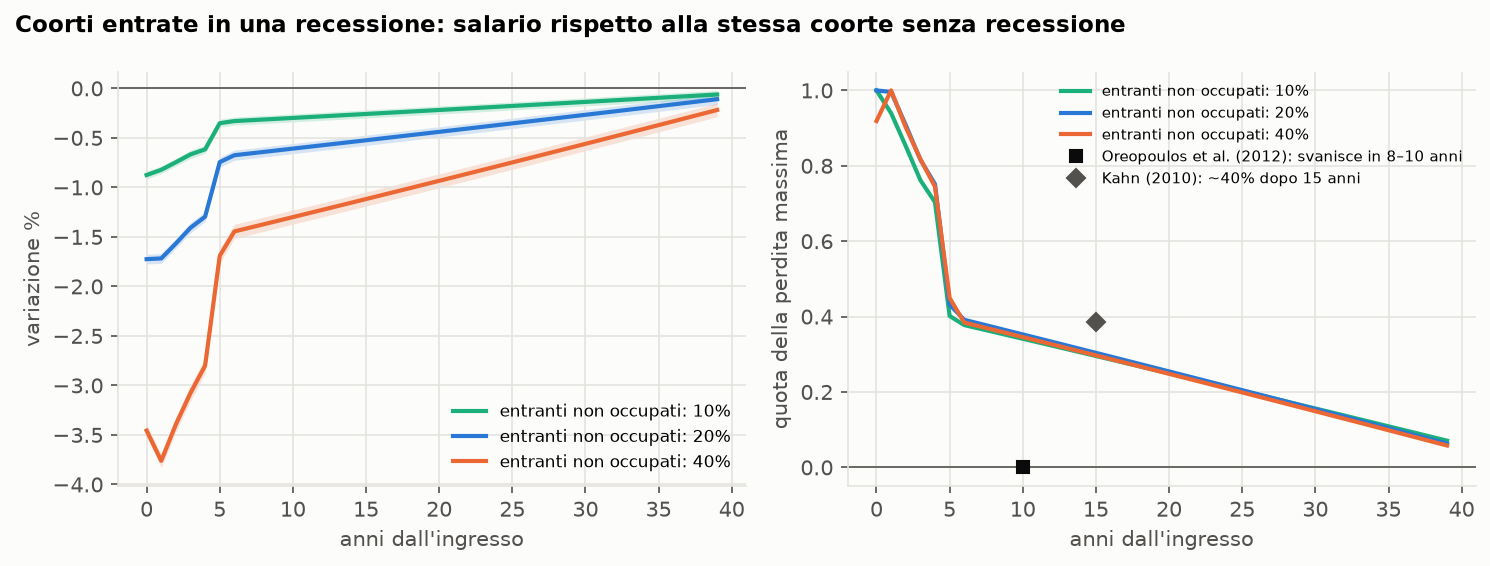
\includegraphics[width=\linewidth]{fig11_coorti_recessione.png}
\caption{Coorti che entrano in una recessione di due anni in cui il 10, 20 o 40 per cento di chi cerca il primo lavoro resta non occupato. (a) Salario medio della coorte rispetto alla stessa coorte senza recessione. (b) Quota della perdita massima che resta, con le evidenze di \citet{Oreopoulos2012} e \citet{Kahn2010}. $N=50.000$, 30 repliche appaiate; le bande sono intervalli di confidenza al 95\%.}\label{fig:recession}
\end{figure}

% ---------------------------------------------------------------------------
\section{Implicazioni per la modellistica aggregata}\label{sec:aggregate}

I modelli di crescita a una equazione restano diffusi, e con buone ragioni. Ci sono lezioni del modello ad agenti che possono esservi incorporate? Sosteniamo che ce ne siano due.

\begin{proposition}[Efficienza emergente dell'apprendimento: un'identità di campo medio]\label{prop:B}
Siano $\bar h^S_{g,t}$ il capitale umano medio dei senior nel gruppo $g$ e $\overline{h^{-1}}^{J}_{g,t}$ la media dell'inverso del capitale umano dei junior nello stesso gruppo, entrambi a inizio periodo $t$. Con abbinamenti casuali dentro i gruppi, il contributo atteso degli incontri all'efficienza dell'apprendimento è
\begin{equation}\label{eq:Bmf}
\mathbb E\big[B^{\mathrm{inc}}_t\big] = \sum_g \frac{J_{g,t}}{J_t}\,\beta\, p^{\mathrm{eff}}_{g,t} \left[\bar h^S_{g,t}\, \overline{h^{-1}}^{J}_{g,t} - 1 + \Omega_{g,t}\right],
\end{equation}
dove
\begin{equation*}
\Omega_{g,t} = \frac{1}{J_{g,t} S_{g,t}}\sum_{j,k\in g}\frac{\max(0,h_{j,t}-h_{k,t})}{h_{j,t}} \ge 0 .
\end{equation*}
\end{proposition}
\begin{proof}
Poiché $\max(0,x) = x + \max(0,-x)$, il guadagno atteso del junior $j$ da un incontro con un senior dello stesso gruppo estratto in modo uniforme è $\beta(\bar h^S_{g,t} - h_{j,t}) + \beta S_{g,t}^{-1}\sum_{k\in g} \max(0, h_{j,t}-h_{k,t})$. Dividendo per $h_{j,t}$, moltiplicando per $p^{\mathrm{eff}}_{g,t}$ e facendo la media sui junior si ottiene il risultato.
\end{proof}

L'Eq.~\eqref{eq:Bmf} è un'identità contabile più che un risultato di comportamento: il suo valore sta in ciò che rende esplicito. È la controparte aggregata delle regole individuali. L'efficienza dell'apprendimento dipende da tre oggetti che una $B$ costante sopprime: le occasioni d'incontro ($p$), la capacità di mentoring rispetto alla domanda ($\kappa S/J$) e la distribuzione della conoscenza tra generazioni ($\bar h^S \overline{h^{-1}}^J$). Nel caso base l'identità è verificata numericamente (0,0437 contro 0,0434 simulato). La dispersione del capitale umano dei junior conta: sostituire $\overline{h^{-1}}^J$ con $1/\bar h^J$ sottostima $B^{\mathrm{inc}}$ di circa il 9 per cento.

\begin{proposition}[Ritardo di trasmissione]\label{prop:lag}
Si supponga che le occasioni d'incontro cambino in modo permanente in $t_0$ e che i senior non imparino dagli incontri. Allora il capitale umano medio dei senior non cambia per $t \le t_0 + s_S - s_J$, e può cambiare da $t_0 + s_S - s_J + 1$ in poi.
\end{proposition}
\begin{proof}
Un lavoratore junior in $t_0$ ha esperienza al massimo $s_J-1$ e diventa senior quando la sua esperienza raggiunge $s_S$, cioè dopo almeno $s_S-s_J+1$ anni. Fino ad allora l'insieme dei senior è composto da lavoratori i cui anni da junior si sono conclusi prima di $t_0$, e il cui capitale umano evolve solo secondo l'Eq.~\eqref{eq:aut}.
\end{proof}

Con $s_J=5$ e $s_S=15$, il capitale umano dei senior resta invariato per dieci anni e il primo effetto compare all'undicesimo, esattamente come nelle simulazioni. La proposizione~\ref{prop:lag} spiega perché le evidenze di primo round sui giovani \citep{Brynjolfsson2025} non possono, da sole, rivelare l'effetto di secondo round sul capitale umano: quest'ultimo resta invisibile per un'intera generazione professionale, e poi si dispiega nel corso di più generazioni. L'elasticità di lungo periodo del capitale umano dei senior alle occasioni d'incontro, $\varepsilon = \Delta \ln \bar h^S_\infty / \Delta\ln p \approx 0{,}10$ nel caso base, svolge qui il ruolo che il grado di isteresi svolge nei modelli aggregati del tasso normale di utilizzo della capacità \citep{Bassi2022}: riassume in un solo numero una proprietà che emerge da comportamenti individuali eterogenei.

% ---------------------------------------------------------------------------
\section{L'introduzione dell'intelligenza artificiale}\label{sec:ai}

\subsection{Specificazione}

L'IA arriva nell'anno $t_0=10$ del periodo registrato. La sua produttività cresce al tasso $g$, e automatizza una quota crescente $\varphi_t$ dei compiti dei lavoratori bersaglio:
\begin{gather}
A_t = (1+g)^{t-t_0}\ \ (t\ge t_0), \qquad \varphi_t = \varphi_{\max}\left(1-\frac{1}{A_t}\right), \label{eq:ai}\\
Y_t = H_t\left[1+\theta\,(A_t-1)\,F_t\right], \label{eq:aiY}
\end{gather}
con $A_t=1$ prima di $t_0$ e $H_t=\sum_i h_{i,t}$. La quota $\varphi_t$ parte da zero e si satura a $\varphi_{\max}$. $F_t\in[0,1]$ è la familiarità con l'IA dei lavoratori che la usano, pesata con il loro capitale umano: chi entra dopo $t_0$ è formato con l'IA, chi c'era già impara a usarla gradualmente. La familiarità non influisce sulla dinamica del capitale umano e vale uno alla fine dell'orizzonte; conta solo per output e salari durante la transizione (appendice~\ref{app:variants}).

Che cosa significa ``sostituire'' un lavoratore? Distinguiamo il bersaglio (junior o senior) dal margine: il lavoratore conserva il posto ma perde compiti, oppure perde il posto. I quattro casi agiscono su parametri diversi della tecnologia degli incontri (tabella~\ref{tab:margins}). Sostituire compiti dei junior moltiplica $p$ per $1-\varphi_t$ (meno occasioni di lavorare accanto a un senior). Sostituire posti dei junior rende ogni anno non occupata una quota $\varphi_t$ dei junior: non incontrano senior né imparano sul lavoro, il loro capitale umano si deprezza al tasso $d$, e l'anno non conta come esperienza, così che restano junior più a lungo e diventano senior più tardi. I loro compiti sono svolti dall'IA, così che l'output corrente non cambia e la perdita opera solo attraverso il capitale umano. Sostituire compiti dei senior moltiplica $\beta$ per $1-\varphi_t$ (ogni incontro trasmette meno); sostituire posti dei senior moltiplica $\kappa$ per $1-\varphi_t$ (meno senior disponibili come mentori). L'IA complementare moltiplica $\beta$ per $1+\varphi_t$ (l'IA rende l'insegnamento più efficace).

\begin{table}[t]\centering\small
\caption{Quattro significati di sostituzione.}\label{tab:margins}
\begin{tabular}{@{}lp{0.36\linewidth}p{0.42\linewidth}@{}}
\toprule
 & Perde compiti & Perde il posto \\
\midrule
Junior & $p\times(1-\varphi_t)$: meno incontri & non occupato con probabilità $\varphi_t$: niente incontri, niente esperienza \\
Senior & $\beta\times(1-\varphi_t)$: meno trasmesso per incontro & $\kappa\times(1-\varphi_t)$: meno mentori \\
\bottomrule
\end{tabular}
\end{table}

Nel testo ci concentriamo su quattro scenari: compiti dei junior, compiti dei senior, posti dei junior e IA complementare. I senior che perdono il posto, i bersagli definiti per qualifica invece che per ruolo, e una variante in cui i junior tengono lo stesso mentore sono discussi nell'appendice~\ref{app:variants}.

Fissiamo $g=0{,}03$ e $\varphi_{\max}=0{,}6$, così che dieci anni dopo la sua introduzione l'IA automatizza il 15 per cento dei compiti bersaglio, in linea con il calo relativo del 13--16 per cento dell'occupazione dei giovani nelle occupazioni esposte \citep{Brynjolfsson2025}; e $\theta=0{,}02$, che dà un guadagno di produttività dello 0,7 per cento in dieci anni, vicino alla stima prudente di \citet{Acemoglu2024}. Poiché $\theta$ non influisce sulla dinamica degli agenti, il sentiero dell'output si può calcolare per qualsiasi $\theta$ a partire da $H_t$, $A_t$ e $F_t$. Ogni scenario condivide i numeri casuali con lo scenario senza IA, così che prima di $t_0$ i due sono identici e tutte le differenze sono dovute all'IA. Usiamo $N=50.000$ e 30 repliche.\footnote{Il modello è invariante alla scala: poiché gli incontri sono estrazioni casuali dentro gruppi grandi e non legami in una rete locale, simulazioni con 5.000 e con 24 milioni di agenti (il numero degli occupati in Italia) danno gli stessi risultati alla quarta cifra; la dimensione della popolazione riduce solo il rumore campionario.}

\subsection{Perdere compiti, perdere il posto}

La tabella~\ref{tab:ai} e la figura~\ref{fig:ai} confrontano i quattro scenari cinquant'anni dopo l'introduzione dell'IA. Sostituire compiti dei junior riduce il capitale umano aggregato del 5,2 per cento e quasi dimezza l'apprendimento dagli incontri. Nei 49 anni tra l'introduzione dell'IA e la fine dell'orizzonte, la perdita equivale a un capitale umano che cresce 0,11 punti percentuali l'anno più lentamente. Il valore cade nell'intervallo di 0,05--0,35 punti che \citet{Ide2026} stima per la crescita di lungo periodo del reddito pro capite, con una differenza: nel nostro modello stazionario la perdita è un effetto di livello che alla lunga si ferma, mentre in quello di Ide è un cambiamento permanente del tasso di crescita. Coerentemente con la proposizione~\ref{prop:lag}, i senior sono colpiti solo dodici anni dopo l'introduzione dell'IA: un anno perché $A_t$ superi uno, più gli undici anni del ritardo di trasmissione.

Sostituire compiti dei senior ha lo stesso effetto medio. Poiché $p$ e $\beta$ entrano nell'apprendimento come prodotto (Eq.~\eqref{eq:Bmf}), ridurre l'uno o l'altro di $1-\varphi_t$ dà la stessa perdita di capitale umano: la differenza appaiata è di 0,002 punti percentuali, con un intervallo di confidenza al 95 per cento che include lo zero. Per lo stock di capitale umano non conta se i junior perdono occasioni per imparare o i senior la capacità di insegnare; conta il prodotto delle due. I canali differiscono per distribuzione e tempi. Meno incontri significa che alcuni junior imparano e altri no, mentre incontri meno efficaci significano che ogni junior impara un po' meno: l'indice di Gini del capitale umano è 0,163 nel primo caso e 0,161 nel secondo. Per i salari conta di più chi usa l'IA: quando l'IA sostituisce compiti dei junior, il suo guadagno va ai lavoratori esperti e il Gini dei salari sale a 0,167; quando sostituisce compiti dei senior, il guadagno va ai lavoratori meno esperti e il Gini dei salari resta a 0,155, come senza IA. Quegli utilizzatori meno esperti sono entrati dopo l'introduzione dell'IA e la conoscono meglio, così che l'output è più alto nella transizione: dieci anni dopo l'introduzione supera il livello senza IA dello 0,35 per cento, contro lo 0,22 per cento quando l'IA sostituisce i junior. Il vantaggio svanisce man mano che chi c'era prima va in pensione, ed è piccolo con $\theta=0{,}02$: il compromesso tra output oggi e capitale umano domani esiste, ma non è lì il grosso della skill cliff.

Se i junior perdono il posto invece dei compiti, la formazione è rinviata, non persa (è lo stesso meccanismo per cui le coorti che entrano nel mercato del lavoro durante una recessione subiscono perdite salariali persistenti \citep{Kahn2010,Oreopoulos2012}): poiché l'esperienza si accumula solo lavorando, un junior non occupato resta junior finché non ha completato cinque anni di lavoro. La perdita di capitale umano (5,7 per cento) è vicina a quella della sostituzione di compiti, ma la sua composizione è diversa: l'ingresso tra i senior è ritardato e le carriere sono più brevi, così che dopo cinquant'anni i senior sono l'11 per cento in meno, mentre il capitale umano medio di chi diventa senior cala solo dell'1,9 per cento.

L'IA complementare è lo specchio della sostituzione di compiti: con la stessa intensità $\varphi_t$, il capitale umano aggregato sale del 5,2 per cento e l'output del 12 per cento dopo cinquant'anni.

\begin{table}[t]\centering\small
\caption{Effetti dell'IA cinquant'anni dopo la sua introduzione, rispetto allo scenario senza IA (media di 30 repliche appaiate). Tutti gli scenari sono nella tabella~\ref{tab:ai_all}.}\label{tab:ai}
\begin{tabular}{@{}lrrrrrr@{}}
\toprule
Bersaglio, margine & $H$ & $h$ senior & $B^{\mathrm{inc}}$ & $Y_{+10}$ & $Y_{+50}$ & Gini \\
\midrule
Junior, compiti ($p$) & $-5{,}2\%$ & $-4{,}5\%$ & $-45\%$ & $+0{,}22\%$ & $+0{,}9\%$ & 0,167 \\
Senior, compiti ($\beta$) & $-5{,}2\%$ & $-4{,}5\%$ & $-45\%$ & $+0{,}35\%$ & $+0{,}9\%$ & 0,155 \\
Junior, posto & $-5{,}7\%$ & $-1{,}9\%$ & $-44\%$ & $+0{,}06\%$ & $+0{,}4\%$ & 0,173 \\
Complementare & $+5{,}2\%$ & $+4{,}3\%$ & $+45\%$ & $+0{,}76\%$ & $+12{,}0\%$ & 0,150 \\
\bottomrule
\multicolumn{7}{@{}p{0.95\linewidth}@{}}{\footnotesize $Y_{+10}$, $Y_{+50}$: output dieci e cinquant'anni dopo l'introduzione dell'IA, $\theta=0{,}02$. Gini: salari a fine orizzonte; 0,155 senza IA. Per i junior non occupati, $B^{\mathrm{inc}}$ è la media su tutti i junior.}
\end{tabular}
\end{table}

\begin{figure}[t]\centering
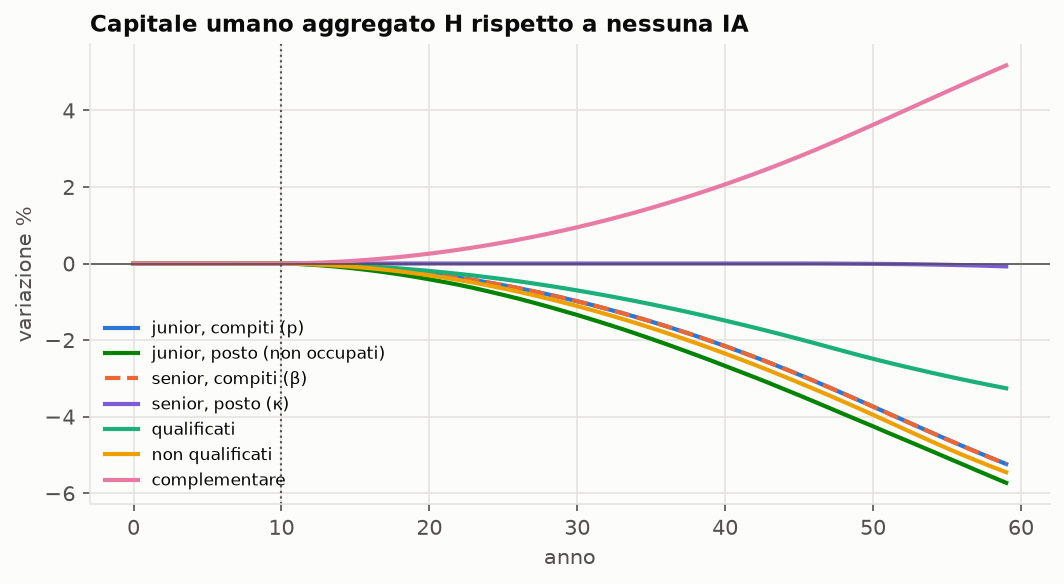
\includegraphics[width=.8\linewidth]{fig6_scenari_H.png}
\caption{Capitale umano aggregato rispetto allo scenario senza IA, per i quattro scenari della tabella~\ref{tab:ai} (la linea tratteggiata, compiti dei senior, quasi coincide con i compiti dei junior). Media su 30 repliche; le bande sono intervalli di confidenza al 95\%.}\label{fig:ai}
\end{figure}

\subsection{La corsa}

L'ipotesi della skill cliff è in fondo una corsa tra la crescita della produttività dell'IA e l'erosione della conoscenza su cui l'IA si regge. Con $\theta=0{,}02$ e bersaglio junior, l'IA da sola aumenterebbe l'output del 6,5 per cento dopo cinquant'anni; con la perdita di capitale umano che induce, il guadagno è dello 0,9 per cento, così che la skill cliff ne assorbe circa l'86 per cento (figura~\ref{fig:race}). La quota assorbita è già il 55 per cento dopo dieci anni e il 73 per cento dopo venticinque: nei primi anni il guadagno dell'IA è più piccolo, perché chi c'era prima non la conosce ancora, mentre la perdita di capitale umano è la stessa. Il valore di pareggio di $\theta$, sotto il quale l'output a fine orizzonte è più basso che senza IA, è 0,017 per $g=0{,}03$, e 0,019 se i junior perdono il posto invece dei compiti. Un'IA più veloce ($g=0{,}06$) causa una perdita di capitale umano maggiore ($-7{,}5$ per cento) ma anche una crescita più rapida di $A_t$, così che il valore di pareggio di $\theta$ scende (0,005): con una produttività dell'IA esponenziale la corsa alla fine si vince, e la domanda diventa su quale orizzonte la si perde.

\begin{figure}[t]\centering
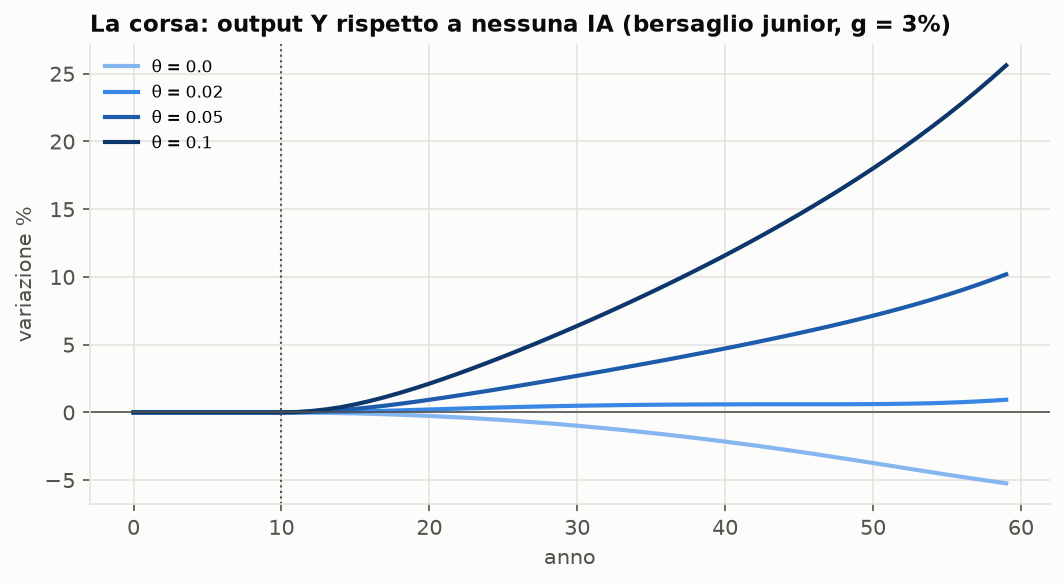
\includegraphics[width=.8\linewidth]{fig8_corsa.png}
\caption{Output rispetto allo scenario senza IA, bersaglio junior, $g=0{,}03$, per diversi valori di $\theta$.}\label{fig:race}
\end{figure}

\subsection{Automazione privata e automazione sociale}

Perché le imprese dovrebbero sostituire i junior oltre ciò che è socialmente desiderabile? Seguendo \citet{Ide2026}, i contratti per la trasmissione della conoscenza tacita sono incompleti: un'impresa che forma un junior non cattura il valore della conoscenza che quel junior trasmetterà in seguito. Lo rappresentiamo confrontando un'impresa e un pianificatore che scelgono una quota costante $\varphi$ di compiti junior automatizzati da $t_0$ in poi. L'output netto rispetto a nessuna automazione è
\begin{equation}\label{eq:d15}
y_t(\varphi) = r_t(\varphi)\left(1+\pi\varphi-\tfrac{c}{2}\varphi^2\right), \qquad r_t(\varphi)=\frac{H_t(\varphi)}{H_t(0)},
\end{equation}
dove $\pi=0{,}10$ è il guadagno dell'automazione completa e $c=1/3$ un costo di adozione. L'impresa prende il capitale umano come dato e sceglie $\varphi=\pi/c=0{,}30$; il pianificatore massimizza $\sum_k \rho^{k+1} y_{t_0+k}(\varphi)$ su un orizzonte dato, con $r_t(\varphi)$ misurato nel modello.

La figura~\ref{fig:d15} mostra che l'impresa automatizza troppo, e che l'eccesso cresce con l'orizzonte del pianificatore. Con $\rho=0{,}97$ la quota ottima è 0,25 su dieci anni, 0,19 su venticinque e 0,09 su cinquanta. Su cinquant'anni la scelta dell'impresa dà un output netto scontato dello 0,6 per cento \emph{inferiore} a quello senza alcuna automazione, contro il $+0{,}14$ per cento dell'ottimo. Su dieci anni, invece, le due scelte quasi coincidono, perché la perdita di capitale umano dei senior si materializza solo dopo il ritardo di trasmissione della proposizione~\ref{prop:lag}: un decisore il cui orizzonte è un bilancio o un ciclo elettorale si comporta quasi come l'impresa. I valori di $\pi$ e $c$ determinano il livello della scelta dell'impresa, non il segno dell'eccesso, che deriva solo dal fatto che l'impresa non vede $r_t(\varphi)$.

\begin{figure}[t]\centering
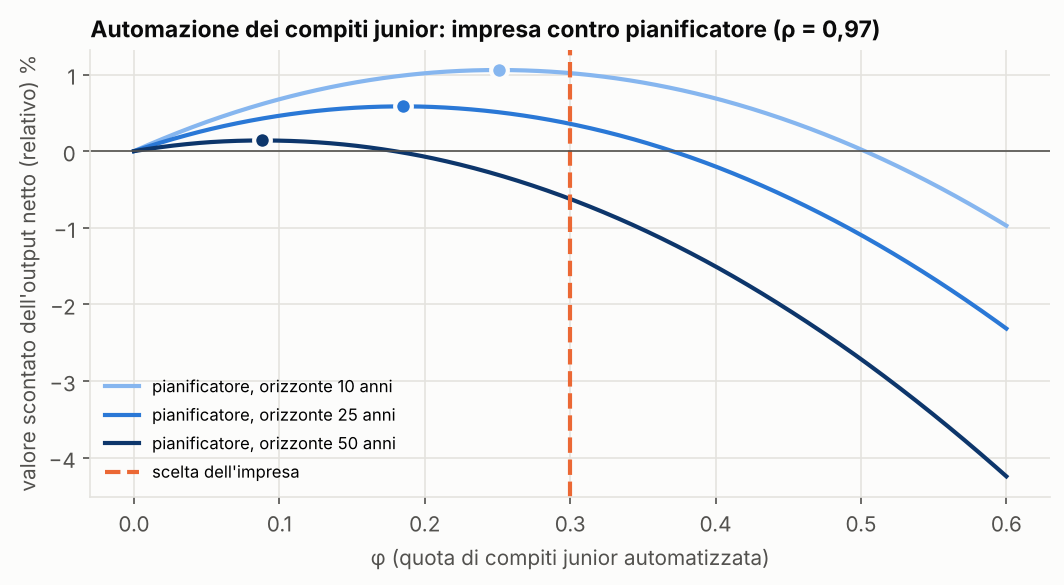
\includegraphics[width=.8\linewidth]{fig10_automazione.png}
\caption{Output netto scontato rispetto a nessuna automazione in funzione della quota automatizzata dei compiti junior, per pianificatori con orizzonti diversi ($\rho=0{,}97$). I punti indicano l'ottimo del pianificatore; la linea tratteggiata la scelta dell'impresa.}\label{fig:d15}
\end{figure}

% ---------------------------------------------------------------------------
\section{Discussione e conclusioni}\label{sec:conclusions}

\subsection{Un fallimento di mercato che nessuno vede}

Quando un'impresa automatizza il lavoro dei junior, i suoi conti migliorano subito: la produttività dei senior sale e i costi scendono. Nessuna voce di bilancio registra che la prossima generazione di lavoratori riceverà meno apprendimento, e nessun indicatore economico coglie la caduta di $B$ che avviene dentro le gerarchie organizzative. La struttura del problema somiglia all'inquinamento: chi inquina ottiene un vantaggio competitivo immediato, mentre chi ne sopporta il costo è disperso nel tempo e nello spazio, e spesso non è ancora nato. La proposizione~\ref{prop:lag} e la sezione~\ref{sec:ai} danno una dimensione quantitativa a questa analogia: nella nostra calibrazione il costo è invisibile nel capitale umano dei senior per dieci anni, un'impresa automatizza più del triplo della quota che sceglierebbe un pianificatore con un orizzonte di cinquant'anni, e quando il costo compare le politiche che avrebbero potuto prevenirlo sono già in ritardo: la formazione di un senior richiede quindici-vent'anni di esposizione a situazioni difficili, e non si può accelerare con sussidi o corsi intensivi.

Le risposte discusse nel dibattito pubblico differiscono per fattibilità e orizzonte. A livello d'impresa, una quota della capacità dei gruppi di lavoro può essere riservata al mentoring e a compiti affidati ai junior. A livello istituzionale, i programmi di apprendistato possono separare la formazione dalla produzione e vincolare senior e junior a lavorare insieme su problemi reali. A livello fiscale, un contributo sull'automazione dei compiti d'ingresso internalizzerebbe l'esternalità individuata da \citet{Ide2026}. Infine, la stessa IA può essere indirizzata a potenziare l'insegnamento dei senior invece di sostituire i junior: è la direzione del progresso tecnico che \citet{Acemoglu2024} auspica. Nel modello queste risposte corrispondono, rispettivamente, ad aumentare $\kappa$, aumentare $p$, tassare le riduzioni di $p$ e aumentare $\beta$, e l'Eq.~\eqref{eq:Bmf} fornisce una metrica comune per confrontarle. La figura~\ref{fig:policies} applica ogni leva dall'introduzione dell'IA con la stessa intensità, il 10 per cento del proprio parametro, e riporta la quota della perdita di capitale umano che recupera.\footnote{Il modello non ha prezzi, quindi la stessa intensità non significa lo stesso costo. L'output non dipende dalla quota automatizzata, quindi il costo in output di un contributo sull'automazione è quello misurato nella sezione~\ref{sec:ai} (figura~\ref{fig:d15}).} La leva giusta dipende da quale vincolo è attivo. Quando l'IA toglie compiti ai junior e i mentori sono abbondanti, gli apprendistati ($p$) e un'IA che aiuta i senior a insegnare ($\beta$) sono equivalenti, come implica la proposizione~\ref{prop:B}: ciascuno recupera più dell'intera perdita nei primi dieci anni, la metà dopo venticinque e un quarto dopo cinquanta, perché la leva è fissa mentre la perdita continua a crescere. Riservare capacità di mentoring ($\kappa$) non recupera nulla, perché la capacità non è vincolante. Quando i senior perdono il posto e i mentori sono scarsi ($\kappa=0{,}1$), l'ordine si inverte: la capacità di mentoring recupera quasi tutta la perdita in dieci anni e un quarto dopo cinquanta, mentre gli apprendistati non recuperano nulla, perché la domanda aggiuntiva di incontri è razionata. Rendere più efficace l'insegnamento funziona in entrambi i casi. Un contributo che riduce del 10 per cento la quota automatizzata recupera il 10 per cento della perdita a ogni orizzonte. Per un decisore pubblico o un'impresa che investe in capitale umano, la prima domanda è quindi empirica: ai junior mancano le occasioni per imparare, o ai senior il tempo per insegnare?

\begin{figure}[t]\centering
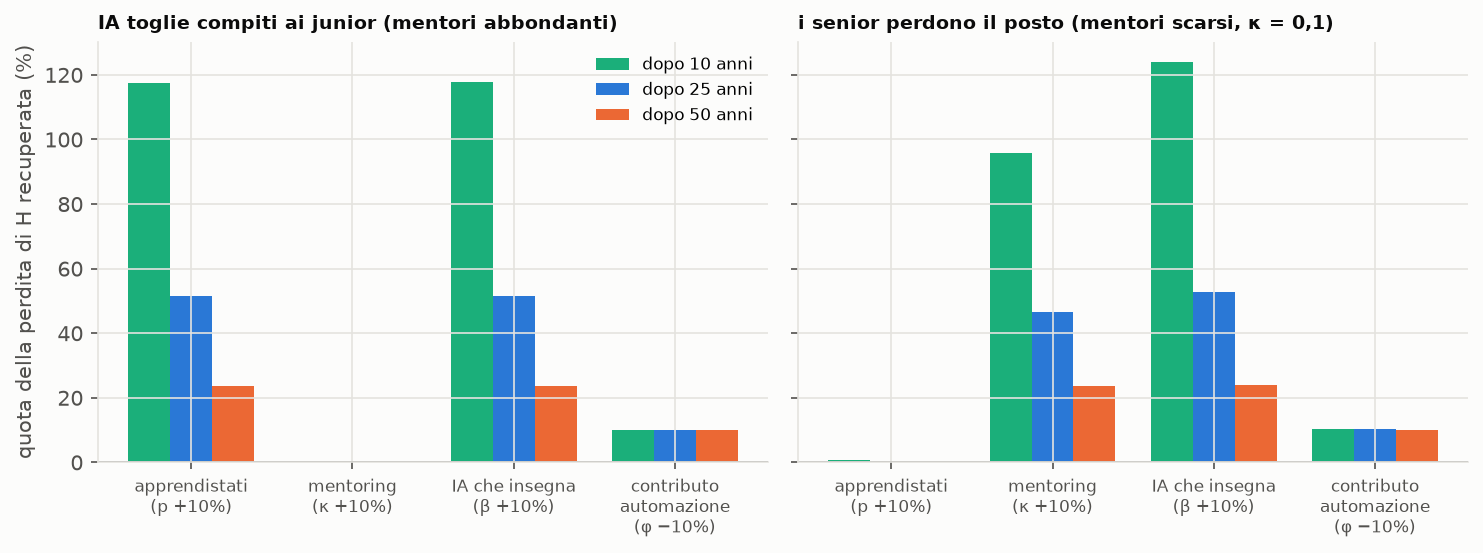
\includegraphics[width=\linewidth]{fig12_politiche.png}
\caption{Quota della perdita di capitale umano aggregato dovuta all'IA che ogni leva recupera, applicata dall'introduzione dell'IA con un'intensità pari al 10 per cento del proprio parametro. A sinistra: l'IA toglie compiti ai junior, la capacità di mentoring è abbondante ($\kappa=0{,}2$). A destra: i senior perdono il posto, la capacità di mentoring è scarsa ($\kappa=0{,}1$). $N=50.000$, 30 repliche appaiate.}\label{fig:policies}
\end{figure}

\subsection{Conclusioni}

Un modello volutamente minimo dell'apprendimento dagli incontri, senza scelte economiche, dà due risultati principali. Una riduzione delle occasioni d'incontro produce una caduta ritardata e cumulativa del capitale umano, una skill cliff, i cui tempi sono governati dalla distanza tra le soglie di junior e senior. E poiché l'apprendimento dipende dal prodotto tra le occasioni d'incontro e la loro efficacia, un'IA che toglie compiti ai junior o ai senior costa lo stesso capitale umano, mentre i due casi differiscono per disuguaglianza e per guadagno di output nella transizione; i junior che perdono il posto rinviano la propria formazione invece di perderla. Ne seguono due conseguenze: un guadagno prudente di produttività dell'IA può essere in gran parte assorbito dalla skill cliff che provoca, e le imprese che non internalizzano la trasmissione della conoscenza automatizzano troppo, di una quantità invisibile su un orizzonte di dieci anni. L'identità aggregata per $B$ rende questi meccanismi disponibili ai modelli di crescita a una equazione.

Al di là di questi contributi, l'analisi lascia aperte diverse direzioni di ricerca. L'IA può anche essere una fonte di apprendimento: l'evidenza che aiuta soprattutto i lavoratori meno esperti \citep{BrynjolfssonLiRaymond2025} suggerisce un canale di tutoraggio che potrebbe compensare una parte della perdita di incontri, o aggravarla se riduce lo sforzo di chi impara \citep{Ide2026}. Le imprese sono rappresentate da un'unica decisione sulla quota automatizzata: imprese eterogenee che competono, formano e si contendono i lavoratori permetterebbero di studiare come si ripartisce l'esternalità. Una variante demografica basata sulla piramide per età italiana, in cui grandi coorti si avvicinano alla pensione, permetterà di separare la scogliera generata dalla demografia da quella aggiunta dall'IA. Infine, l'erosione delle competenze può interagire con la distribuzione della ricchezza, se l'accesso agli strumenti di produzione prende sempre più la forma di rendite ricorrenti.

La matematica non dice che $B$ debba cadere. Dice che cosa succede se glielo si permette.

\section*{Contributi degli autori (CRediT)}
\textbf{Federico Bassi:} \todo{da definire}. \textbf{Vincenzo Lio:} concettualizzazione, metodologia, software, stesura originale.

\section*{Disponibilità dei dati}
Codice, file di configurazione e dati simulati sono disponibili su \url{https://github.com/ViciusLio/skill-cliff-abm}.

\appendix
\section{Protocollo ODD}\label{app:odd}

Questa appendice descrive il modello secondo il protocollo ODD (Overview, Design concepts, Details) nella versione aggiornata da \citet{Grimm2020}. Si riferisce all'implementazione nel repository (pacchetto \texttt{skillcliff}); i valori dei parametri sono quelli della tabella~\ref{tab:params} e del file \texttt{base.yaml}.

\subsection{Scopo e regolarità}
Il modello studia come l'efficienza dell'apprendimento, $B$, emerga dagli incontri tra lavoratori junior e senior, e come una riduzione di quegli incontri, in particolare la sostituzione del lavoro dei junior con l'IA, agisca sul capitale umano nel tempo. È valutato rispetto a tre regolarità: un profilo salariale per età concavo che cresce lentamente e si appiattisce, come nel settore privato italiano; una quota di apprendimento dai colleghi pari al 4--9 per cento dei salari dei junior \citep{Jarosch2021}; e una distribuzione stazionaria del capitale umano in assenza di shock.

\subsection{Entità, variabili di stato e scale}
Gli unici agenti sono i lavoratori. Ogni lavoratore $i$ ha un identificativo, un'età $a_i$ (anni), un'esperienza $s_i$ (anni di occupazione dall'ingresso), una qualifica $q_i\in\{L,H\}$ e un capitale umano $h_i\ge 0$; negli scenari con IA anche una familiarità con l'IA $f_i\in[0,1]$ e, nella variante con mentore stabile, l'identificativo del mentore corrente. Il ruolo (junior se $s_i<s_J$, senior se $s_i\ge s_S$, intermedio altrimenti) deriva dall'esperienza. Lo stato globale è costituito dall'indice temporale $t$ e, negli scenari con IA, dalla produttività dell'IA $A_t$ e dalla quota automatizzata $\varphi_t$. Non ci sono spazio né rete: le interazioni sono estrazioni casuali dentro i gruppi di qualifica. Un passo temporale è un anno; una simulazione consiste in un burn-in di 300 anni, che elimina la dipendenza dalle condizioni iniziali, seguito da 60 anni registrati. La popolazione ha dimensione costante $N$ (5.000 nella fase~1, 50.000 negli esperimenti con IA); i risultati sono invarianti rispetto a $N$ a meno del rumore campionario.

\subsection{Panoramica dei processi e ordine di esecuzione}
In ogni anno i processi seguenti sono eseguiti in quest'ordine, ciascuno su tutti gli agenti insieme (aggiornamento sincrono):
\begin{enumerate}
\item \emph{Invecchiamento}: $a_i$ aumenta di uno; $s_i$ aumenta di uno, e $f_i$ viene aggiornata, se il lavoratore era occupato l'anno precedente.
\item \emph{Pensionamento}: escono i lavoratori con $a_i\ge\bar a$.
\item \emph{Ingresso}: entrano tanti lavoratori quanti ne sono usciti, con $s=0$.
\item \emph{Ruoli}: junior e senior sono identificati in base all'esperienza.
\item \emph{IA} (solo sezione~\ref{sec:ai}): i moltiplicatori di $p$, $\kappa$ e $\beta$ per ogni gruppo di qualifica sono calcolati da $\varphi_t$; quando i junior perdono il posto, una quota $\varphi_t$ dei junior bersaglio è estratta come non occupata.
\item \emph{Incontri}: dentro ogni gruppo di qualifica, i junior occupati incontrano un senior con probabilità $p^{\mathrm{eff}}_{g,t}$ e calcolano il loro guadagno, Eq.~\eqref{eq:peff}--\eqref{eq:meeting}.
\item \emph{Apprendimento autonomo e obsolescenza}: Eq.~\eqref{eq:aut}; i junior non occupati si deprezzano soltanto.
\item \emph{Aggiornamento}: tutti i guadagni, calcolati sul capitale umano di inizio anno, sono sommati insieme.
\item \emph{Osservazione}: si registrano le statistiche aggregate (dopo il burn-in).
\end{enumerate}

\subsection{Concetti di progettazione}
\emph{Principi di base.} L'efficienza dell'apprendimento come risultato degli incontri \citep{LucasMoll2014}, l'apprendimento sul ciclo di vita \citep{BenPorath1967}, e sostituzione contro complementarità dell'IA \citep{Acemoglu2024,Ide2026}.
\emph{Emergenza.} L'efficienza dell'apprendimento $B$, il profilo salariale per età, la disuguaglianza dei salari e i tempi degli effetti di una riduzione degli incontri emergono dai singoli incontri; il ritardo di trasmissione (proposizione~\ref{prop:lag}) e la dipendenza di $B$ dalla distribuzione della conoscenza (proposizione~\ref{prop:B}) sono proprietà emergenti che caratterizziamo analiticamente.
\emph{Adattamento, obiettivi, apprendimento, previsione.} I lavoratori seguono regole fisse e non prendono decisioni; non si adattano, non ottimizzano e non prevedono. L'unica decisione è la quota automatizzata della sezione~\ref{sec:ai}, presa fuori dal modello ad agenti confrontando sentieri simulati (impresa contro pianificatore).
\emph{Percezione.} Un junior osserva solo il capitale umano del senior incontrato.
\emph{Interazione.} Diretta e asimmetrica: la conoscenza passa dal senior al junior, mai in senso inverso, e solo dentro lo stesso gruppo di qualifica. Le interazioni sono razionate dalla capacità di mentoring $\kappa S_g$.
\emph{Stocasticità.} La qualifica e il capitale umano iniziale degli entranti, il verificarsi degli incontri, la scelta del senior e, quando i junior perdono il posto, la non occupazione sono casuali. Ogni replica usa un proprio seed, derivato da un seed radice; flussi di numeri casuali separati sono usati per demografia, incontri e IA, così che scenari con lo stesso seed condividono tutte le estrazioni fino all'arrivo dell'IA (numeri casuali comuni).
\emph{Collettivi.} Nessuno oltre ai gruppi di qualifica e ai ruoli.
\emph{Osservazione.} Ogni anno: numero di junior, senior e incontri; probabilità d'incontro effettiva; capitale umano aggregato $H_t$ e output $Y_t$; capitale umano medio per ruolo, età e qualifica; $B_t$ e le sue componenti; il coefficiente di Gini dei salari. Le statistiche sono medie su 30 repliche, con intervalli di confidenza al 95 per cento basati sulla $t$ di Student.

\subsection{Inizializzazione}
Si creano $N$ lavoratori con una qualifica estratta con probabilità $q$ e un'esperienza estratta in modo uniforme sulla carriera del proprio gruppo di qualifica; l'età deriva dall'esperienza e dall'età d'ingresso, e il capitale umano è estratto come per gli entranti. Il burn-in di 300 anni rende i risultati indipendenti da questo stato iniziale: con 300 anni invece di 120 la deriva residua del capitale umano medio scende da $10^{-4}$ a meno di $10^{-5}$ l'anno, e i confronti tra scenari cambiano di meno di 0,1 punti percentuali.

\subsection{Dati in ingresso}
Il modello non usa serie storiche in ingresso. I parametri sono letti da un file di configurazione; negli scenari con IA, $A_t$ e $\varphi_t$ sono funzioni deterministiche del tempo, Eq.~\eqref{eq:ai}.

\subsection{Sottomodelli}
\emph{Ingresso}: Eq.~\eqref{eq:entry}, con età d'ingresso 20 o 25 a seconda della qualifica. \emph{Incontri}: Eq.~\eqref{eq:peff} e \eqref{eq:meeting}, applicate dentro ogni gruppo di qualifica; il senior è estratto in modo uniforme. \emph{Apprendimento autonomo e obsolescenza}: Eq.~\eqref{eq:aut}. \emph{Output e salari}: $Y_t=\sum_i h_{i,t}$ e $w_i=h_i$ senza IA; Eq.~\eqref{eq:aiY} con l'IA, con salari e familiarità come descritti nell'appendice~\ref{app:variants}. \emph{IA}: Eq.~\eqref{eq:ai} e i moltiplicatori descritti nella sezione~\ref{sec:ai}; quando i junior perdono il posto, un junior bersaglio è non occupato con probabilità $\varphi_t$, in modo indipendente ogni anno, e quell'anno non conta come esperienza. \emph{Impresa contro pianificatore}: Eq.~\eqref{eq:d15}, valutata su una griglia di quote automatizzate.

\subsection{Implementazione e verifica}
Il modello è scritto in Python con operazioni NumPy vettorizzate (un array per variabile di stato). Una batteria di test automatici verifica, tra l'altro, che il numero di agenti si conservi, che il capitale umano non sia mai negativo, che $p=0$ implichi nessun apprendimento dagli incontri, che simulazioni con lo stesso seed siano identiche, che ogni incontro abbini un junior a un senior della stessa qualifica, e che tutti gli scenari con IA coincidano con lo scenario senza IA prima di $t_0$. Un'implementazione indipendente a oggetti in Mesa riproduce i risultati entro $\pm1$ per cento (appendice~\ref{app:docking}). Codice, configurazione e dati sono disponibili su \url{https://github.com/ViciusLio/skill-cliff-abm}.

\section{Varianti degli scenari con IA}\label{app:variants}

La tabella~\ref{tab:ai_all} riporta tutti gli scenari simulati. Questa appendice discute quelli che non sono nel testo.

\begin{table}[t]\centering\small
\caption{Effetti dell'IA cinquant'anni dopo la sua introduzione in tutti gli scenari, rispetto allo scenario senza IA (media di 30 repliche appaiate).}\label{tab:ai_all}
\begin{tabular}{@{}lrrrrrr@{}}
\toprule
Bersaglio, margine & $H$ & $h$ senior & $B^{\mathrm{inc}}$ & $Y_{+10}$ & $Y_{+50}$ & Gini \\
\midrule
Junior, compiti ($p$) & $-5{,}2\%$ & $-4{,}5\%$ & $-45\%$ & $+0{,}22\%$ & $+0{,}9\%$ & 0,167 \\
Junior, posto & $-5{,}7\%$ & $-1{,}9\%$ & $-44\%$ & $+0{,}06\%$ & $+0{,}4\%$ & 0,173 \\
Senior, compiti ($\beta$) & $-5{,}2\%$ & $-4{,}5\%$ & $-45\%$ & $+0{,}35\%$ & $+0{,}9\%$ & 0,155 \\
Senior, posto ($\kappa$) & $-0{,}1\%$ & $0{,}0\%$ & $-2\%$ & $+0{,}62\%$ & $+6{,}4\%$ & 0,149 \\
Non qualificati, compiti & $-5{,}5\%$ & $-5{,}0\%$ & $-49\%$ & $+0{,}18\%$ & $+0{,}7\%$ & 0,169 \\
Qualificati, compiti & $-3{,}3\%$ & $-2{,}9\%$ & $-21\%$ & $+0{,}30\%$ & $+3{,}0\%$ & 0,153 \\
Complementare & $+5{,}2\%$ & $+4{,}3\%$ & $+45\%$ & $+0{,}76\%$ & $+12{,}0\%$ & 0,150 \\
\bottomrule
\multicolumn{7}{@{}p{0.95\linewidth}@{}}{\footnotesize $Y_{+10}$, $Y_{+50}$: output dieci e cinquant'anni dopo l'introduzione dell'IA, $\theta=0{,}02$. Gini: salari a fine orizzonte; 0,155 senza IA. Senior che perdono il posto con capacità di mentoring più scarsa ($\kappa=0{,}1$): $H$ $-4{,}8\%$. Per i junior non occupati, $B^{\mathrm{inc}}$ è la media su tutti i junior.}
\end{tabular}
\end{table}

\subsection{I senior che perdono il posto}

I senior che perdono il posto sono quasi innocui nel caso base, ma solo perché la capacità di mentoring è abbondante: con $S/J\approx5{,}7$ ci sono più mentori potenziali di quanti ne servano, e il vincolo dell'Eq.~\eqref{eq:peff} diventa attivo solo circa trent'anni dopo l'introduzione dell'IA. Quando la capacità è più scarsa, la stessa sostituzione conta (tabella~\ref{tab:kappa}). Con $\kappa=0{,}1$, dove il vincolo è appena attivo, riduce il capitale umano aggregato del 4,8 per cento, quasi quanto la sostituzione di compiti; con $\kappa=0{,}05$ la perdita è minore (2,3 per cento) perché gli incontri sono già scarsi senza IA, così che c'è meno da perdere. Quanti senior facciano davvero da mentori è quindi una grandezza empirica cruciale. Sostituire compiti dei senior, che agisce su $\beta$, non dipende da $\kappa$.

\begin{table}[h]\centering\small
\caption{Senior che perdono il posto: sensibilità alla capacità di mentoring (cinquant'anni dopo l'introduzione dell'IA, 30 repliche).}\label{tab:kappa}
\begin{tabular}{@{}lrrr@{}}
\toprule
$\kappa$ & $p^{\mathrm{eff}}$ senza IA & $H$ & $h$ senior \\
\midrule
0,05 & 0,29 & $-2{,}3\%$ & $-2{,}0\%$ \\
0,10 & 0,57 & $-4{,}8\%$ & $-4{,}2\%$ \\
0,20 (base) & 0,60 & $-0{,}1\%$ & $0{,}0\%$ \\
\bottomrule
\end{tabular}
\end{table}

\subsection{Bersagli definiti per qualifica}

Quando l'IA sostituisce lavoratori qualificati o non qualificati, il taglio dei junior e quello dei senior si applicano dentro il gruppo corrispondente. Sostituire i non qualificati costa più che sostituire i qualificati ($-5{,}5$ contro $-3{,}3$ per cento di capitale umano aggregato) e aumenta la disuguaglianza salariale (Gini 0,169 contro 0,153), soprattutto perché i non qualificati sono il 70 per cento degli entranti. Poiché questi scenari tagliano sia $p$ sia $\beta$ dentro il gruppo, l'apprendimento nel gruppo scala con $(1-\varphi_t)^2$: non sono direttamente confrontabili con gli scenari per ruolo.

\subsection{Familiarità con l'IA}

Il guadagno dell'IA dipende da quanto la conoscono i lavoratori che la usano, $U_t$: i lavoratori non sostituiti (i non junior se l'IA sostituisce i junior, i non senior se sostituisce i senior, il gruppo di qualifica colpito negli scenari per qualifica, tutti per l'IA complementare). Ogni lavoratore ha una familiarità $f_i\in[0,1]$: chi entra dopo $t_0$ è formato con l'IA e ha $f_i=1$; chi c'era già parte da $f_i=0$ e, per ogni anno di lavoro con l'IA, aggiorna $f_i \leftarrow f_i+\gamma(1-f_i)$, con $\gamma=0{,}1$. $F_t=\sum_{i\in U}h_if_i/\sum_{i\in U}h_i$ è la familiarità degli utilizzatori, pesata con il capitale umano. Gli utilizzatori guadagnano $w_i=h_i[1+\theta(A_t-1)f_i]$ e gli altri lavoratori $w_i=h_i$; il resto dell'output, $\theta(A_t-1)F_t(H_t-\sum_{i\in U}h_i)$, è una rendita che va ai proprietari dell'IA. Il livello del guadagno è quindi proporzionale a tutto il capitale umano, compreso quello incorporato nei compiti che l'IA svolge al posto dei lavoratori sostituiti, mentre i suoi utilizzatori determinano con quanta efficacia viene sfruttato; con $f_i=1$ per tutti i lavoratori l'Eq.~\eqref{eq:aiY} si riduce alla forma usata senza familiarità, così che $\theta$ conserva la sua interpretazione per l'intera economia. La familiarità non influisce sull'apprendimento, quindi cambia output e salari ma non la dinamica del capitale umano; poiché alla fine dell'orizzonte tutti i lavoratori sono entrati dopo $t_0$, $F_t=1$ cinquant'anni dopo l'introduzione dell'IA.

La velocità $\gamma$ con cui chi c'era già impara a usare l'IA conta solo nella transizione. Dieci anni dopo l'introduzione dell'IA, l'output supera il livello senza IA dello 0,07 per cento quando l'IA sostituisce compiti dei junior e dello 0,30 per cento quando sostituisce compiti dei senior se $\gamma=0{,}05$; dello 0,36 e dello 0,40 per cento se $\gamma=0{,}2$; e dello 0,42 per cento in entrambi i casi se $\gamma=1$, cioè senza familiarità. Venticinque anni dopo l'introduzione le differenze sono quasi scomparse.

\subsection{Mentore stabile}

Nel caso base un junior incontra ogni anno un senior estratto a caso. In una variante, un junior che incontra un senior tiene quel mentore finché entrambi restano occupati e il junior resta junior, a meno che la coppia non si sciolga con probabilità annua $\lambda$; le coppie occupano capacità di mentoring, e $\lambda=1$ riproduce esattamente il caso base. Con $\lambda=0{,}15$, vicino al tasso annuo di separazione dei giovani lavoratori, e $\beta$ ricalibrato (da 0,10 a 0,075) per mantenere $B^{\mathrm{inc}}$ al valore della fase~1, il profilo salariale per età, la quota di apprendimento dagli incontri e il Gini dei salari restano praticamente invariati, e il ritardo di trasmissione della proposizione~\ref{prop:lag} è ancora di undici anni. La proposizione~\ref{prop:B} diventa un'approssimazione, che sovrastima $B^{\mathrm{inc}}$ di circa il 5 per cento perché i junior abbinati non sono un campione casuale. La simmetria tra $p$ e $\beta$ si rompe: poiché $p$ governa solo la formazione di nuove coppie, sostituire compiti dei junior riduce il capitale umano aggregato del 3,5 per cento, contro il 5,3 per cento quando si sostituiscono compiti dei senior; sostituire posti dei junior costa il 7,2 per cento, perché un junior che esce dall'occupazione perde anche il mentore. La variante cambia le grandezze, non i tempi né il segno degli effetti.

\section{Analisi di sensibilità globale}\label{app:sobol}

Diversi parametri sono scelti a mano (tabella~\ref{tab:params}). Ne facciamo quindi variare nove insieme, su intervalli ampi ($p\in[0{,}3;0{,}9]$, $\kappa\in[0{,}1;0{,}4]$, $\beta\in[0{,}05;0{,}15]$, $\sigma\in[0{,}1;0{,}3]$, $\delta_0\in[0{,}03;0{,}05]$, $S_h\in[40;60]$, $d\in[0{,}008;0{,}016]$ e, per l'IA, $g\in[0{,}01;0{,}05]$ e $\varphi_{\max}\in[0{,}4;0{,}8]$), e calcoliamo indici di sensibilità basati sulla varianza (di Sobol) \citep{Sobol2001,Saltelli2008} per tre risultati: l'apprendimento dagli incontri nel caso base, la perdita di capitale umano aggregato cinquant'anni dopo che l'IA toglie compiti ai junior, e l'eccesso di automazione della sezione~\ref{sec:ai} ($\rho=0{,}97$, orizzonte di cinquant'anni). Usiamo 64 punti base quasi casuali, cioè 704 vettori di parametri, con $N=5.000$ e una replica ciascuno; gli intervalli di confidenza sono ottenuti con il bootstrap. Le soglie $s_J$ e $s_S$ restano fisse: per la proposizione~\ref{prop:lag} il ritardo di trasmissione dipende solo da loro.

I segni dei risultati principali non dipendono dai parametri. Su tutti i 704 vettori la perdita di capitale umano non è mai positiva (il 90 per cento dei valori è tra $-11{,}6$ e $-1{,}2$ per cento) e l'eccesso di automazione è sempre positivo (il 90 per cento tra 0,06 e 0,30). I loro livelli dipendono soprattutto da $p$, $\beta$ e $\delta_0$, i cui indici totali sono compresi tra 0,23 e 0,35 (figura~\ref{fig:sobol}); i parametri dell'IA, $g$ e $\varphi_{\max}$, spiegano circa un quarto della varianza della perdita di capitale umano e nulla dell'eccesso di automazione, che è calcolato per una quota automatizzata costante. Gli indici del primo ordine sono molto più piccoli di quelli totali: i parametri agiscono insieme, come la proposizione~\ref{prop:B} implica per $p$ e $\beta$, che entrano nell'apprendimento come prodotto. La dispersione del capitale umano all'ingresso, $\sigma$, è irrilevante, e la capacità di mentoring, $\kappa$, conta poco, perché nella maggior parte dello spazio dei parametri non è vincolante.

\begin{figure}[h]\centering
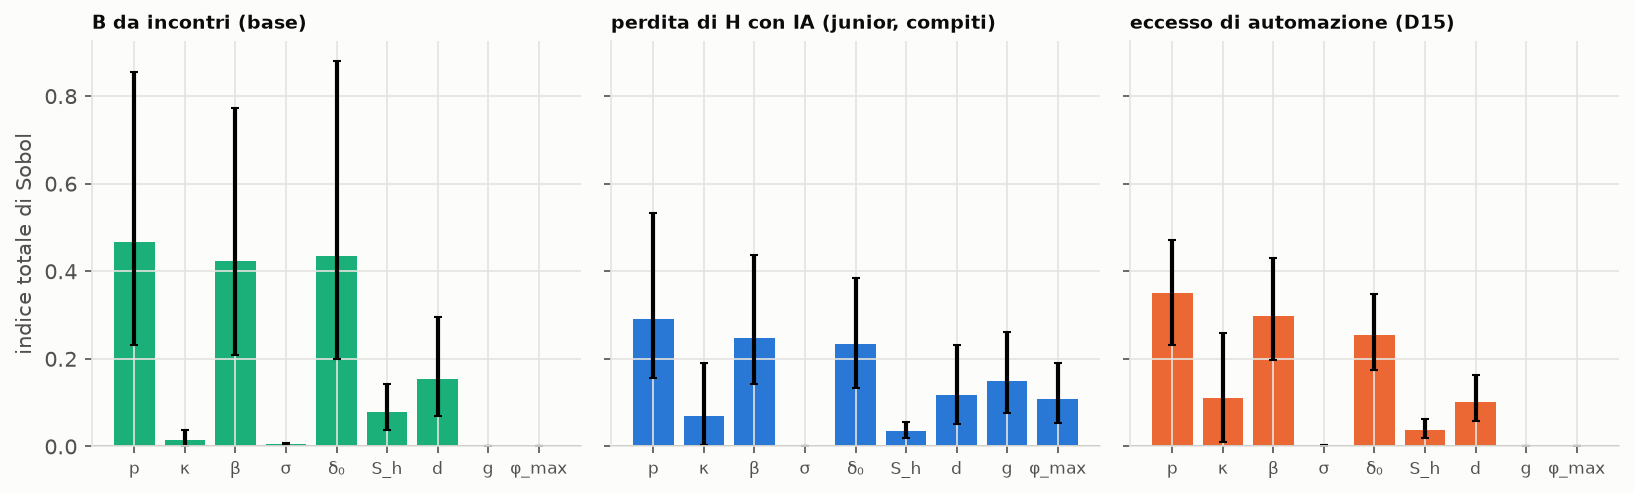
\includegraphics[width=\linewidth]{fig13_sensibilita_sobol.png}
\caption{Indici totali di Sobol di tre risultati rispetto a nove parametri (704 vettori di parametri, $N=5.000$). Le barre sono intervalli di confidenza bootstrap al 95\%.}\label{fig:sobol}
\end{figure}

\section{Docking con un'implementazione indipendente}\label{app:docking}

La tabella~\ref{tab:docking} confronta il modello vettorizzato con un'implementazione indipendente in Mesa (un oggetto per agente), con $N=5.000$ e 30 repliche ciascuno, come nella fase~1. Per ogni statistica si riportano due test. Il test di Welch ha come ipotesi nulla che le due implementazioni abbiano la stessa media: un $p$-value \emph{grande} significa che non si rileva alcuna differenza. Poiché non rilevare una differenza non prova l'equivalenza, eseguiamo anche un test di equivalenza (due test unilaterali, TOST) con un margine di $\pm1$ per cento della media, scelto ben al di sotto del più piccolo effetto che interpretiamo (circa $-2$ per cento): qui l'ipotesi nulla è che la differenza superi il margine, e un $p$-value \emph{piccolo} dimostra l'equivalenza. L'intervallo di confidenza al 90 per cento della differenza relativa indica il margine più stretto entro cui l'equivalenza vale al livello del 5 per cento.

\begin{table}[h]\centering\small
\caption{Docking: implementazione vettorizzata (NumPy) contro implementazione a oggetti (Mesa) ($N=5.000$, 30 repliche ciascuna).}\label{tab:docking}
\resizebox{\linewidth}{!}{%
\begin{tabular}{@{}lrrrrrr@{}}
\toprule
Statistica & NumPy & Mesa & Diff.\ rel. & $p$ (Welch) & IC 90\% diff.\ rel. & $p$ (TOST, $\pm1\%$) \\
\midrule
$h$ medio & 1,9929 & 1,9920 & $-0{,}04\%$ & 0,56 & $[-0{,}17\%;\ +0{,}08\%]$ & $<0{,}001$ \\
$h$ medio dei junior & 1,4184 & 1,4179 & $-0{,}04\%$ & 0,64 & $[-0{,}17\%;\ +0{,}10\%]$ & $<0{,}001$ \\
$h$ medio dei senior & 2,1667 & 2,1657 & $-0{,}05\%$ & 0,55 & $[-0{,}19\%;\ +0{,}09\%]$ & $<0{,}001$ \\
$B^{\mathrm{inc}}$ & 0,0429 & 0,0429 & $-0{,}06\%$ & 0,75 & $[-0{,}36\%;\ +0{,}24\%]$ & $<0{,}001$ \\
$B^{\mathrm{aut}}$ & 0,0264 & 0,0264 & $0{,}00\%$ & 0,32 & $[-0{,}00\%;\ +0{,}00\%]$ & $<0{,}001$ \\
\bottomrule
\end{tabular}}
\end{table}

La variante con mentore stabile della sezione~\ref{sec:ai} è stata sottoposta allo stesso docking, con l'implementazione in Mesa estesa alle coppie persistenti ($\lambda=0{,}15$, $\beta=0{,}075$). L'equivalenza entro $\pm1$ per cento è dimostrata per tutte e cinque le statistiche ($p_{\mathrm{TOST}}\le0{,}001$); le differenze relative sono comprese tra $-0{,}40$ e $0$ per cento con 30 repliche e tra $-0{,}12$ e $+0{,}05$ per cento in una seconda esecuzione con 60 repliche e un seed radice diverso ($p$ tra 0,35 e 0,93 nel test di Welch).

Una terza implementazione in NetLogo \citep{Wilensky1999}, scritta per i coautori e i lettori che lavorano con quel software, copre l'intero modello della sezione~\ref{sec:ai}: il caso base, le quattro combinazioni di bersaglio e margine, l'IA complementare e la variante con mentore stabile. Con 30 repliche per parte, l'equivalenza entro $\pm1$ per cento è dimostrata per ogni statistica e ogni scenario, e la massima differenza relativa tra le medie è dello 0,25 per cento (file \texttt{report/numeri\_netlogo.json} nel repository).

\bibliographystyle{elsarticle-harv}
\bibliography{../references}

\end{document}
